% **************************************************************************************************************
% A Classic Thesis Style
% An Homage to The Elements of Typographic Style
%
% Copyright (C) 2017 André Miede and Ivo Pletikosić
%
% If you like the style then I would appreciate a postcard. My address
% can be found in the file ClassicThesis.pdf. A collection of the
% postcards I received so far is available online at
% http://postcards.miede.de
%
% License:
% This program is free software; you can redistribute it and/or modify
% it under the terms of the GNU General Public License as published by
% the Free Software Foundation; either version 2 of the License, or
% (at your option) any later version.
%
% This program is distributed in the hope that it will be useful,
% but WITHOUT ANY WARRANTY; without even the implied warranty of
% MERCHANTABILITY or FITNESS FOR A PARTICULAR PURPOSE.  See the
% GNU General Public License for more details.
%
% You should have received a copy of the GNU General Public License
% along with this program; see the file COPYING.  If not, write to
% the Free Software Foundation, Inc., 59 Temple Place - Suite 330,
% Boston, MA 02111-1307, USA.
%
% PLEASE SEE ALSO THE AUTHORS' NOTE REGARDING THIS LICENSE
% IN THE DOCUMENTATION (ClassicThesis.pdf --> Chapter 1 / Chapter01.tex)
% **************************************************************************************************************
\RequirePackage{silence} % :-\
    \WarningFilter{scrreprt}{Usage of package `titlesec'}
    %\WarningFilter{scrreprt}{Activating an ugly workaround}
    \WarningFilter{titlesec}{Non standard sectioning command detected}
\documentclass[ twoside,openright,titlepage,numbers=noenddot,%1headlines,
                headinclude,footinclude,cleardoublepage=empty,
                BCOR=5mm,paper=a4,fontsize=11pt,table
                ]{scrreprt}

%********************************************************************
% Note: Make all your adjustments in here
%*******************************************************
% ****************************************************************************************************
% classicthesis-config.tex
% formerly known as loadpackages.sty, classicthesis-ldpkg.sty, and classicthesis-preamble.sty
% Use it at the beginning of your ClassicThesis.tex, or as a LaTeX Preamble
% in your ClassicThesis.{tex,lyx} with % ****************************************************************************************************
% classicthesis-config.tex
% formerly known as loadpackages.sty, classicthesis-ldpkg.sty, and classicthesis-preamble.sty
% Use it at the beginning of your ClassicThesis.tex, or as a LaTeX Preamble
% in your ClassicThesis.{tex,lyx} with % ****************************************************************************************************
% classicthesis-config.tex
% formerly known as loadpackages.sty, classicthesis-ldpkg.sty, and classicthesis-preamble.sty
% Use it at the beginning of your ClassicThesis.tex, or as a LaTeX Preamble
% in your ClassicThesis.{tex,lyx} with \input{classicthesis-config}
% ****************************************************************************************************
% If you like the classicthesis, then I would appreciate a postcard.
% My address can be found in the file ClassicThesis.pdf. A collection
% of the postcards I received so far is available online at
% http://postcards.miede.de
% ****************************************************************************************************


% ****************************************************************************************************
% 0. Set the encoding of your files. UTF-8 is the only sensible encoding nowadays. If you can't read
% äöüßáéçèê∂åëæƒÏ€ then change the encoding setting in your editor, not the line below. If your editor
% does not support utf8 use another editor!
% ****************************************************************************************************
\PassOptionsToPackage{utf8}{inputenc}
  \usepackage{inputenc}

% ****************************************************************************************************
% 1. Configure classicthesis for your needs here, e.g., remove "drafting" below
% in order to deactivate the time-stamp on the pages
% (see ClassicThesis.pdf for more information):
% ****************************************************************************************************
\PassOptionsToPackage{
  drafting=true,    % print version information on the bottom of the pages
  tocaligned=false, % the left column of the toc will be aligned (no indentation)
  dottedtoc=false,  % page numbers in ToC flushed right
  parts=true,       % use part division
  eulerchapternumbers=true, % use AMS Euler for chapter font (otherwise Palatino)
  linedheaders=false,       % chaper headers will have line above and beneath
  floatperchapter=true,     % numbering per chapter for all floats (i.e., Figure 1.1)
  eulermath=false,  % use awesome Euler fonts for mathematical formulae (only with pdfLaTeX)
  beramono=true,    % toggle a nice monospaced font (w/ bold)
  % palatino=false,   % deactivate standard font for loading another one, see the last section at the end of this file for suggestions
}{classicthesis}


% ****************************************************************************************************
% 2. Personal data and user ad-hoc commands
% ****************************************************************************************************
\newcommand{\myTitle}{Uberfuzz\xspace}
\newcommand{\mySubtitle}{A Cooperative Fuzzing Framework\xspace}
\newcommand{\myDegree}{M.Sc. Artificial Intelligence\xspace}
\newcommand{\myName}{Andrea Jemmett\xspace}
\newcommand{\myProf}{Dr. Sanjay Rawat\xspace}
\newcommand{\myOtherProf}{Put name here\xspace}
\newcommand{\mySupervisor}{Put name here\xspace}
\newcommand{\myFaculty}{Faculty of Science\xspace}
\newcommand{\myDepartment}{Dept. of Computer Science\xspace}
\newcommand{\myUni}{Vrije Universiteit Amsterdam\xspace}
\newcommand{\myLocation}{Amsterdam, Netherlands\xspace}
\newcommand{\myTime}{January 2018\xspace}
\newcommand{\myVersion}{version 4.5}

% ********************************************************************
% Setup, finetuning, and useful commands
% ********************************************************************
\newcounter{dummy} % necessary for correct hyperlinks (to index, bib, etc.)
\newlength{\abcd} % for ab..z string length calculation
\providecommand{\mLyX}{L\kern-.1667em\lower.25em\hbox{Y}\kern-.125emX\@}
\newcommand{\ie}{i.\,e.}
\newcommand{\Ie}{I.\,e.}
\newcommand{\eg}{e.\,g.}
\newcommand{\Eg}{E.\,g.}
% ****************************************************************************************************


% ****************************************************************************************************
% 3. Loading some handy packages
% ****************************************************************************************************
% ********************************************************************
% Packages with options that might require adjustments
% ********************************************************************
\PassOptionsToPackage{american}{babel} % change this to your language(s), main language last
% Spanish languages need extra options in order to work with this template
%\PassOptionsToPackage{spanish,es-lcroman}{babel}
    \usepackage{babel}

\usepackage{csquotes}
\PassOptionsToPackage{%
  %backend=biber,bibencoding=utf8, %instead of bibtex
  backend=bibtex8,bibencoding=ascii,%
  language=auto,%
  style=numeric-comp,%
  %style=authoryear-comp, % Author 1999, 2010
  %bibstyle=authoryear,dashed=false, % dashed: substitute rep. author with ---
  sorting=nyt, % name, year, title
  maxbibnames=10, % default: 3, et al.
  %backref=true,%
  natbib=true % natbib compatibility mode (\citep and \citet still work)
}{biblatex}
    \usepackage{biblatex}

\PassOptionsToPackage{fleqn}{amsmath}       % math environments and more by the AMS
  \usepackage{amsmath}

% ********************************************************************
% General useful packages
% ********************************************************************
\PassOptionsToPackage{inline}{enumitem}
  \usepackage{enumitem}
\PassOptionsToPackage{linesnumbered,commentsnumbered,ruled}{algorithm2e}
  \usepackage{algorithm2e}
\usepackage{setspace}
\usepackage{lipsum}
\PassOptionsToPackage{T1}{fontenc} % T2A for cyrillics
  \usepackage{fontenc}
\usepackage{textcomp} % fix warning with missing font shapes
\usepackage{scrhack} % fix warnings when using KOMA with listings package
\usepackage{xspace} % to get the spacing after macros right
\usepackage{mparhack} % get marginpar right
%\usepackage{fixltx2e} % fixes some LaTeX stuff --> since 2015 in the LaTeX kernel (see below)
% \usepackage[latest]{latexrelease} % emulate newer kernel version if older is detected
\PassOptionsToPackage{printonlyused,smaller}{acronym}
  \usepackage{acronym} % nice macros for handling all acronyms in the thesis
  %\renewcommand{\bflabel}[1]{{#1}\hfill} % fix the list of acronyms --> no longer working
  %\renewcommand*{\acsfont}[1]{\textsc{#1}}
  %\renewcommand*{\aclabelfont}[1]{\acsfont{#1}}
  %\def\bflabel#1{{#1\hfill}}
  \def\bflabel#1{{\acsfont{#1}\hfill}}
  \def\aclabelfont#1{\acsfont{#1}}
% ****************************************************************************************************
%\usepackage{pgfplots} % External TikZ/PGF support (thanks to Andreas Nautsch)
%\usetikzlibrary{external}
%\tikzexternalize[mode=list and make, prefix=ext-tikz/]
% ****************************************************************************************************


% ****************************************************************************************************
% 4. Setup floats: tables, (sub)figures, and captions
% ****************************************************************************************************
\usepackage{tabularx} % better tables
  \setlength{\extrarowheight}{3pt} % increase table row height
\newcommand{\tableheadline}[1]{\multicolumn{1}{l}{\spacedlowsmallcaps{#1}}}
\newcommand{\myfloatalign}{\centering} % to be used with each float for alignment
\usepackage{caption}
% Thanks to cgnieder and Claus Lahiri
% http://tex.stackexchange.com/questions/69349/spacedlowsmallcaps-in-caption-label
% [REMOVED DUE TO OTHER PROBLEMS, SEE ISSUE #82]
%\DeclareCaptionLabelFormat{smallcaps}{\bothIfFirst{#1}{~}\MakeTextLowercase{\textsc{#2}}}
%\captionsetup{font=small,labelformat=smallcaps} % format=hang,
\captionsetup{font=small} % format=hang,
\usepackage{subfig}
% ****************************************************************************************************


% ****************************************************************************************************
% 5. Setup code listings
% ****************************************************************************************************
\usepackage{listings}
%\lstset{emph={trueIndex,root},emphstyle=\color{BlueViolet}}%\underbar} % for special keywords
\lstset{language={C},
  keywordstyle=\color{RoyalBlue},%\bfseries,
  basicstyle=\small\ttfamily,
  %identifierstyle=\color{NavyBlue},
  commentstyle=\color{Green}\ttfamily,
  stringstyle=\rmfamily,
  numbers=none,%left,%
  numberstyle=\scriptsize,%\tiny
  stepnumber=5,
  numbersep=8pt,
  showstringspaces=false,
  breaklines=true,
  %frameround=ftff,
  frame=single,
  captionpos=b,
  belowcaptionskip=.75\baselineskip
  %frame=L
}
% ****************************************************************************************************


% ****************************************************************************************************
% 6. PDFLaTeX, hyperreferences, and citation backreferences
% ****************************************************************************************************
% ********************************************************************
% Using PDFLaTeX
% ********************************************************************
\PassOptionsToPackage{hyperfootnotes=false,pdfpagelabels}{hyperref}
  \usepackage{hyperref}  % backref linktocpage pagebackref
  \usepackage{graphicx}


% ********************************************************************
% Hyperreferences
% ********************************************************************
\hypersetup{%
  %draft, % hyperref's draft mode, for printing see below
  colorlinks=true, linktocpage=true, pdfstartpage=3, pdfstartview=FitV,%
  % uncomment the following line if you want to have black links (e.g., for printing)
  %colorlinks=false, linktocpage=false, pdfstartpage=3, pdfstartview=FitV, pdfborder={0 0 0},%
  breaklinks=true, pdfpagemode=UseNone, pageanchor=true, pdfpagemode=UseOutlines,%
  plainpages=false, bookmarksnumbered, bookmarksopen=true, bookmarksopenlevel=1,%
  hypertexnames=true, pdfhighlight=/O,%nesting=true,%frenchlinks,%
  urlcolor=webbrown, linkcolor=RoyalBlue, citecolor=webgreen, %pagecolor=RoyalBlue,%
  %urlcolor=Black, linkcolor=Black, citecolor=Black, %pagecolor=Black,%
  pdftitle={\myTitle},%
  pdfauthor={\textcopyright\ \myName, \myUni, \myFaculty},%
  pdfsubject={},%
  pdfkeywords={},%
  pdfcreator={pdfLaTeX},%
  pdfproducer={LaTeX with hyperref and classicthesis}%
}

% ********************************************************************
% Setup autoreferences
% ********************************************************************
% There are some issues regarding autorefnames
% http://www.ureader.de/msg/136221647.aspx
% http://www.tex.ac.uk/cgi-bin/texfaq2html?label=latexwords
% you have to redefine the makros for the
% language you use, e.g., american, ngerman
% (as chosen when loading babel/AtBeginDocument)
% ********************************************************************
\makeatletter
\@ifpackageloaded{babel}%
  {%
    \addto\extrasamerican{%
      \renewcommand*{\figureautorefname}{Figure}%
      \renewcommand*{\tableautorefname}{Table}%
      \renewcommand*{\partautorefname}{Part}%
      \renewcommand*{\chapterautorefname}{Chapter}%
      \renewcommand*{\sectionautorefname}{Section}%
      \renewcommand*{\subsectionautorefname}{Section}%
      \renewcommand*{\subsubsectionautorefname}{Section}%
    }%
    \addto\extrasngerman{%
      \renewcommand*{\paragraphautorefname}{Absatz}%
      \renewcommand*{\subparagraphautorefname}{Unterabsatz}%
      \renewcommand*{\footnoteautorefname}{Fu\"snote}%
      \renewcommand*{\FancyVerbLineautorefname}{Zeile}%
      \renewcommand*{\theoremautorefname}{Theorem}%
      \renewcommand*{\appendixautorefname}{Anhang}%
      \renewcommand*{\equationautorefname}{Gleichung}%
      \renewcommand*{\itemautorefname}{Punkt}%
    }%
      % Fix to getting autorefs for subfigures right (thanks to Belinda Vogt for changing the definition)
      \providecommand{\subfigureautorefname}{\figureautorefname}%
    }{\relax}
\makeatother


% ****************************************************************************************************
% 7. Last calls before the bar closes
% ****************************************************************************************************
% ********************************************************************
% Development Stuff
% ********************************************************************
\listfiles
%\PassOptionsToPackage{l2tabu,orthodox,abort}{nag}
%  \usepackage{nag}
%\PassOptionsToPackage{warning, all}{onlyamsmath}
%  \usepackage{onlyamsmath}

% ********************************************************************
% Last, but not least...
% ********************************************************************
\usepackage{classicthesis}
% ****************************************************************************************************


% ****************************************************************************************************
% 8. Further adjustments (experimental)
% ****************************************************************************************************
% ********************************************************************
% Changing the text area
% ********************************************************************
%\areaset[current]{312pt}{761pt} % 686 (factor 2.2) + 33 head + 42 head \the\footskip
%\setlength{\marginparwidth}{7em}%
%\setlength{\marginparsep}{2em}%

% ********************************************************************
% Using different fonts
% ********************************************************************
%\usepackage[oldstylenums]{kpfonts} % oldstyle notextcomp
% \usepackage[osf]{libertine}
%\usepackage[light,condensed,math]{iwona}
%\renewcommand{\sfdefault}{iwona}
%\usepackage{lmodern} % <-- no osf support :-(
%\usepackage{cfr-lm} %
%\usepackage[urw-garamond]{mathdesign} <-- no osf support :-(
%\usepackage[default,osfigures]{opensans} % scale=0.95
%\usepackage[sfdefault]{FiraSans}
% \usepackage[opticals,mathlf]{MinionPro} % onlytext
% ********************************************************************
%\usepackage[largesc,osf]{newpxtext}
%\linespread{1.05} % a bit more for Palatino
% Used to fix these:
% https://bitbucket.org/amiede/classicthesis/issues/139/italics-in-pallatino-capitals-chapter
% https://bitbucket.org/amiede/classicthesis/issues/45/problema-testatine-su-classicthesis-style
% ********************************************************************
% ****************************************************************************************************

% adjust colour of acronyms
\makeatletter
\AtBeginDocument{%
    \renewcommand*{\AC@hyperlink}[2]{%
        \begingroup
        \hypersetup{hidelinks}%
        \hyperlink{#1}{#2}%
        \endgroup
    }%
}
\makeatother

% inline enumeration lists
\newlist{enumeratein}{enumerate*}{1}
\setlist[enumeratein]{label=(\roman*)}


% ****************************************************************************************************
% If you like the classicthesis, then I would appreciate a postcard.
% My address can be found in the file ClassicThesis.pdf. A collection
% of the postcards I received so far is available online at
% http://postcards.miede.de
% ****************************************************************************************************


% ****************************************************************************************************
% 0. Set the encoding of your files. UTF-8 is the only sensible encoding nowadays. If you can't read
% äöüßáéçèê∂åëæƒÏ€ then change the encoding setting in your editor, not the line below. If your editor
% does not support utf8 use another editor!
% ****************************************************************************************************
\PassOptionsToPackage{utf8}{inputenc}
  \usepackage{inputenc}

% ****************************************************************************************************
% 1. Configure classicthesis for your needs here, e.g., remove "drafting" below
% in order to deactivate the time-stamp on the pages
% (see ClassicThesis.pdf for more information):
% ****************************************************************************************************
\PassOptionsToPackage{
  drafting=true,    % print version information on the bottom of the pages
  tocaligned=false, % the left column of the toc will be aligned (no indentation)
  dottedtoc=false,  % page numbers in ToC flushed right
  parts=true,       % use part division
  eulerchapternumbers=true, % use AMS Euler for chapter font (otherwise Palatino)
  linedheaders=false,       % chaper headers will have line above and beneath
  floatperchapter=true,     % numbering per chapter for all floats (i.e., Figure 1.1)
  eulermath=false,  % use awesome Euler fonts for mathematical formulae (only with pdfLaTeX)
  beramono=true,    % toggle a nice monospaced font (w/ bold)
  % palatino=false,   % deactivate standard font for loading another one, see the last section at the end of this file for suggestions
}{classicthesis}


% ****************************************************************************************************
% 2. Personal data and user ad-hoc commands
% ****************************************************************************************************
\newcommand{\myTitle}{Uberfuzz\xspace}
\newcommand{\mySubtitle}{A Cooperative Fuzzing Framework\xspace}
\newcommand{\myDegree}{M.Sc. Artificial Intelligence\xspace}
\newcommand{\myName}{Andrea Jemmett\xspace}
\newcommand{\myProf}{Dr. Sanjay Rawat\xspace}
\newcommand{\myOtherProf}{Put name here\xspace}
\newcommand{\mySupervisor}{Put name here\xspace}
\newcommand{\myFaculty}{Faculty of Science\xspace}
\newcommand{\myDepartment}{Dept. of Computer Science\xspace}
\newcommand{\myUni}{Vrije Universiteit Amsterdam\xspace}
\newcommand{\myLocation}{Amsterdam, Netherlands\xspace}
\newcommand{\myTime}{January 2018\xspace}
\newcommand{\myVersion}{version 4.5}

% ********************************************************************
% Setup, finetuning, and useful commands
% ********************************************************************
\newcounter{dummy} % necessary for correct hyperlinks (to index, bib, etc.)
\newlength{\abcd} % for ab..z string length calculation
\providecommand{\mLyX}{L\kern-.1667em\lower.25em\hbox{Y}\kern-.125emX\@}
\newcommand{\ie}{i.\,e.}
\newcommand{\Ie}{I.\,e.}
\newcommand{\eg}{e.\,g.}
\newcommand{\Eg}{E.\,g.}
% ****************************************************************************************************


% ****************************************************************************************************
% 3. Loading some handy packages
% ****************************************************************************************************
% ********************************************************************
% Packages with options that might require adjustments
% ********************************************************************
\PassOptionsToPackage{american}{babel} % change this to your language(s), main language last
% Spanish languages need extra options in order to work with this template
%\PassOptionsToPackage{spanish,es-lcroman}{babel}
    \usepackage{babel}

\usepackage{csquotes}
\PassOptionsToPackage{%
  %backend=biber,bibencoding=utf8, %instead of bibtex
  backend=bibtex8,bibencoding=ascii,%
  language=auto,%
  style=numeric-comp,%
  %style=authoryear-comp, % Author 1999, 2010
  %bibstyle=authoryear,dashed=false, % dashed: substitute rep. author with ---
  sorting=nyt, % name, year, title
  maxbibnames=10, % default: 3, et al.
  %backref=true,%
  natbib=true % natbib compatibility mode (\citep and \citet still work)
}{biblatex}
    \usepackage{biblatex}

\PassOptionsToPackage{fleqn}{amsmath}       % math environments and more by the AMS
  \usepackage{amsmath}

% ********************************************************************
% General useful packages
% ********************************************************************
\PassOptionsToPackage{inline}{enumitem}
  \usepackage{enumitem}
\PassOptionsToPackage{linesnumbered,commentsnumbered,ruled}{algorithm2e}
  \usepackage{algorithm2e}
\usepackage{setspace}
\usepackage{lipsum}
\PassOptionsToPackage{T1}{fontenc} % T2A for cyrillics
  \usepackage{fontenc}
\usepackage{textcomp} % fix warning with missing font shapes
\usepackage{scrhack} % fix warnings when using KOMA with listings package
\usepackage{xspace} % to get the spacing after macros right
\usepackage{mparhack} % get marginpar right
%\usepackage{fixltx2e} % fixes some LaTeX stuff --> since 2015 in the LaTeX kernel (see below)
% \usepackage[latest]{latexrelease} % emulate newer kernel version if older is detected
\PassOptionsToPackage{printonlyused,smaller}{acronym}
  \usepackage{acronym} % nice macros for handling all acronyms in the thesis
  %\renewcommand{\bflabel}[1]{{#1}\hfill} % fix the list of acronyms --> no longer working
  %\renewcommand*{\acsfont}[1]{\textsc{#1}}
  %\renewcommand*{\aclabelfont}[1]{\acsfont{#1}}
  %\def\bflabel#1{{#1\hfill}}
  \def\bflabel#1{{\acsfont{#1}\hfill}}
  \def\aclabelfont#1{\acsfont{#1}}
% ****************************************************************************************************
%\usepackage{pgfplots} % External TikZ/PGF support (thanks to Andreas Nautsch)
%\usetikzlibrary{external}
%\tikzexternalize[mode=list and make, prefix=ext-tikz/]
% ****************************************************************************************************


% ****************************************************************************************************
% 4. Setup floats: tables, (sub)figures, and captions
% ****************************************************************************************************
\usepackage{tabularx} % better tables
  \setlength{\extrarowheight}{3pt} % increase table row height
\newcommand{\tableheadline}[1]{\multicolumn{1}{l}{\spacedlowsmallcaps{#1}}}
\newcommand{\myfloatalign}{\centering} % to be used with each float for alignment
\usepackage{caption}
% Thanks to cgnieder and Claus Lahiri
% http://tex.stackexchange.com/questions/69349/spacedlowsmallcaps-in-caption-label
% [REMOVED DUE TO OTHER PROBLEMS, SEE ISSUE #82]
%\DeclareCaptionLabelFormat{smallcaps}{\bothIfFirst{#1}{~}\MakeTextLowercase{\textsc{#2}}}
%\captionsetup{font=small,labelformat=smallcaps} % format=hang,
\captionsetup{font=small} % format=hang,
\usepackage{subfig}
% ****************************************************************************************************


% ****************************************************************************************************
% 5. Setup code listings
% ****************************************************************************************************
\usepackage{listings}
%\lstset{emph={trueIndex,root},emphstyle=\color{BlueViolet}}%\underbar} % for special keywords
\lstset{language={C},
  keywordstyle=\color{RoyalBlue},%\bfseries,
  basicstyle=\small\ttfamily,
  %identifierstyle=\color{NavyBlue},
  commentstyle=\color{Green}\ttfamily,
  stringstyle=\rmfamily,
  numbers=none,%left,%
  numberstyle=\scriptsize,%\tiny
  stepnumber=5,
  numbersep=8pt,
  showstringspaces=false,
  breaklines=true,
  %frameround=ftff,
  frame=single,
  captionpos=b,
  belowcaptionskip=.75\baselineskip
  %frame=L
}
% ****************************************************************************************************


% ****************************************************************************************************
% 6. PDFLaTeX, hyperreferences, and citation backreferences
% ****************************************************************************************************
% ********************************************************************
% Using PDFLaTeX
% ********************************************************************
\PassOptionsToPackage{hyperfootnotes=false,pdfpagelabels}{hyperref}
  \usepackage{hyperref}  % backref linktocpage pagebackref
  \usepackage{graphicx}


% ********************************************************************
% Hyperreferences
% ********************************************************************
\hypersetup{%
  %draft, % hyperref's draft mode, for printing see below
  colorlinks=true, linktocpage=true, pdfstartpage=3, pdfstartview=FitV,%
  % uncomment the following line if you want to have black links (e.g., for printing)
  %colorlinks=false, linktocpage=false, pdfstartpage=3, pdfstartview=FitV, pdfborder={0 0 0},%
  breaklinks=true, pdfpagemode=UseNone, pageanchor=true, pdfpagemode=UseOutlines,%
  plainpages=false, bookmarksnumbered, bookmarksopen=true, bookmarksopenlevel=1,%
  hypertexnames=true, pdfhighlight=/O,%nesting=true,%frenchlinks,%
  urlcolor=webbrown, linkcolor=RoyalBlue, citecolor=webgreen, %pagecolor=RoyalBlue,%
  %urlcolor=Black, linkcolor=Black, citecolor=Black, %pagecolor=Black,%
  pdftitle={\myTitle},%
  pdfauthor={\textcopyright\ \myName, \myUni, \myFaculty},%
  pdfsubject={},%
  pdfkeywords={},%
  pdfcreator={pdfLaTeX},%
  pdfproducer={LaTeX with hyperref and classicthesis}%
}

% ********************************************************************
% Setup autoreferences
% ********************************************************************
% There are some issues regarding autorefnames
% http://www.ureader.de/msg/136221647.aspx
% http://www.tex.ac.uk/cgi-bin/texfaq2html?label=latexwords
% you have to redefine the makros for the
% language you use, e.g., american, ngerman
% (as chosen when loading babel/AtBeginDocument)
% ********************************************************************
\makeatletter
\@ifpackageloaded{babel}%
  {%
    \addto\extrasamerican{%
      \renewcommand*{\figureautorefname}{Figure}%
      \renewcommand*{\tableautorefname}{Table}%
      \renewcommand*{\partautorefname}{Part}%
      \renewcommand*{\chapterautorefname}{Chapter}%
      \renewcommand*{\sectionautorefname}{Section}%
      \renewcommand*{\subsectionautorefname}{Section}%
      \renewcommand*{\subsubsectionautorefname}{Section}%
    }%
    \addto\extrasngerman{%
      \renewcommand*{\paragraphautorefname}{Absatz}%
      \renewcommand*{\subparagraphautorefname}{Unterabsatz}%
      \renewcommand*{\footnoteautorefname}{Fu\"snote}%
      \renewcommand*{\FancyVerbLineautorefname}{Zeile}%
      \renewcommand*{\theoremautorefname}{Theorem}%
      \renewcommand*{\appendixautorefname}{Anhang}%
      \renewcommand*{\equationautorefname}{Gleichung}%
      \renewcommand*{\itemautorefname}{Punkt}%
    }%
      % Fix to getting autorefs for subfigures right (thanks to Belinda Vogt for changing the definition)
      \providecommand{\subfigureautorefname}{\figureautorefname}%
    }{\relax}
\makeatother


% ****************************************************************************************************
% 7. Last calls before the bar closes
% ****************************************************************************************************
% ********************************************************************
% Development Stuff
% ********************************************************************
\listfiles
%\PassOptionsToPackage{l2tabu,orthodox,abort}{nag}
%  \usepackage{nag}
%\PassOptionsToPackage{warning, all}{onlyamsmath}
%  \usepackage{onlyamsmath}

% ********************************************************************
% Last, but not least...
% ********************************************************************
\usepackage{classicthesis}
% ****************************************************************************************************


% ****************************************************************************************************
% 8. Further adjustments (experimental)
% ****************************************************************************************************
% ********************************************************************
% Changing the text area
% ********************************************************************
%\areaset[current]{312pt}{761pt} % 686 (factor 2.2) + 33 head + 42 head \the\footskip
%\setlength{\marginparwidth}{7em}%
%\setlength{\marginparsep}{2em}%

% ********************************************************************
% Using different fonts
% ********************************************************************
%\usepackage[oldstylenums]{kpfonts} % oldstyle notextcomp
% \usepackage[osf]{libertine}
%\usepackage[light,condensed,math]{iwona}
%\renewcommand{\sfdefault}{iwona}
%\usepackage{lmodern} % <-- no osf support :-(
%\usepackage{cfr-lm} %
%\usepackage[urw-garamond]{mathdesign} <-- no osf support :-(
%\usepackage[default,osfigures]{opensans} % scale=0.95
%\usepackage[sfdefault]{FiraSans}
% \usepackage[opticals,mathlf]{MinionPro} % onlytext
% ********************************************************************
%\usepackage[largesc,osf]{newpxtext}
%\linespread{1.05} % a bit more for Palatino
% Used to fix these:
% https://bitbucket.org/amiede/classicthesis/issues/139/italics-in-pallatino-capitals-chapter
% https://bitbucket.org/amiede/classicthesis/issues/45/problema-testatine-su-classicthesis-style
% ********************************************************************
% ****************************************************************************************************

% adjust colour of acronyms
\makeatletter
\AtBeginDocument{%
    \renewcommand*{\AC@hyperlink}[2]{%
        \begingroup
        \hypersetup{hidelinks}%
        \hyperlink{#1}{#2}%
        \endgroup
    }%
}
\makeatother

% inline enumeration lists
\newlist{enumeratein}{enumerate*}{1}
\setlist[enumeratein]{label=(\roman*)}


% ****************************************************************************************************
% If you like the classicthesis, then I would appreciate a postcard.
% My address can be found in the file ClassicThesis.pdf. A collection
% of the postcards I received so far is available online at
% http://postcards.miede.de
% ****************************************************************************************************


% ****************************************************************************************************
% 0. Set the encoding of your files. UTF-8 is the only sensible encoding nowadays. If you can't read
% äöüßáéçèê∂åëæƒÏ€ then change the encoding setting in your editor, not the line below. If your editor
% does not support utf8 use another editor!
% ****************************************************************************************************
\PassOptionsToPackage{utf8}{inputenc}
  \usepackage{inputenc}

% ****************************************************************************************************
% 1. Configure classicthesis for your needs here, e.g., remove "drafting" below
% in order to deactivate the time-stamp on the pages
% (see ClassicThesis.pdf for more information):
% ****************************************************************************************************
\PassOptionsToPackage{
  drafting=true,    % print version information on the bottom of the pages
  tocaligned=false, % the left column of the toc will be aligned (no indentation)
  dottedtoc=false,  % page numbers in ToC flushed right
  parts=true,       % use part division
  eulerchapternumbers=true, % use AMS Euler for chapter font (otherwise Palatino)
  linedheaders=false,       % chaper headers will have line above and beneath
  floatperchapter=true,     % numbering per chapter for all floats (i.e., Figure 1.1)
  eulermath=false,  % use awesome Euler fonts for mathematical formulae (only with pdfLaTeX)
  beramono=true,    % toggle a nice monospaced font (w/ bold)
  % palatino=false,   % deactivate standard font for loading another one, see the last section at the end of this file for suggestions
}{classicthesis}


% ****************************************************************************************************
% 2. Personal data and user ad-hoc commands
% ****************************************************************************************************
\newcommand{\myTitle}{Uberfuzz\xspace}
\newcommand{\mySubtitle}{A Cooperative Fuzzing Framework\xspace}
\newcommand{\myDegree}{M.Sc. Artificial Intelligence\xspace}
\newcommand{\myName}{Andrea Jemmett\xspace}
\newcommand{\myProf}{Dr. Sanjay Rawat\xspace}
\newcommand{\myOtherProf}{Put name here\xspace}
\newcommand{\mySupervisor}{Put name here\xspace}
\newcommand{\myFaculty}{Faculty of Science\xspace}
\newcommand{\myDepartment}{Dept. of Computer Science\xspace}
\newcommand{\myUni}{Vrije Universiteit Amsterdam\xspace}
\newcommand{\myLocation}{Amsterdam, Netherlands\xspace}
\newcommand{\myTime}{January 2018\xspace}
\newcommand{\myVersion}{version 4.5}

% ********************************************************************
% Setup, finetuning, and useful commands
% ********************************************************************
\newcounter{dummy} % necessary for correct hyperlinks (to index, bib, etc.)
\newlength{\abcd} % for ab..z string length calculation
\providecommand{\mLyX}{L\kern-.1667em\lower.25em\hbox{Y}\kern-.125emX\@}
\newcommand{\ie}{i.\,e.}
\newcommand{\Ie}{I.\,e.}
\newcommand{\eg}{e.\,g.}
\newcommand{\Eg}{E.\,g.}
% ****************************************************************************************************


% ****************************************************************************************************
% 3. Loading some handy packages
% ****************************************************************************************************
% ********************************************************************
% Packages with options that might require adjustments
% ********************************************************************
\PassOptionsToPackage{american}{babel} % change this to your language(s), main language last
% Spanish languages need extra options in order to work with this template
%\PassOptionsToPackage{spanish,es-lcroman}{babel}
    \usepackage{babel}

\usepackage{csquotes}
\PassOptionsToPackage{%
  %backend=biber,bibencoding=utf8, %instead of bibtex
  backend=bibtex8,bibencoding=ascii,%
  language=auto,%
  style=numeric-comp,%
  %style=authoryear-comp, % Author 1999, 2010
  %bibstyle=authoryear,dashed=false, % dashed: substitute rep. author with ---
  sorting=nyt, % name, year, title
  maxbibnames=10, % default: 3, et al.
  %backref=true,%
  natbib=true % natbib compatibility mode (\citep and \citet still work)
}{biblatex}
    \usepackage{biblatex}

\PassOptionsToPackage{fleqn}{amsmath}       % math environments and more by the AMS
  \usepackage{amsmath}

% ********************************************************************
% General useful packages
% ********************************************************************
\PassOptionsToPackage{inline}{enumitem}
  \usepackage{enumitem}
\PassOptionsToPackage{linesnumbered,commentsnumbered,ruled}{algorithm2e}
  \usepackage{algorithm2e}
\usepackage{setspace}
\usepackage{lipsum}
\PassOptionsToPackage{T1}{fontenc} % T2A for cyrillics
  \usepackage{fontenc}
\usepackage{textcomp} % fix warning with missing font shapes
\usepackage{scrhack} % fix warnings when using KOMA with listings package
\usepackage{xspace} % to get the spacing after macros right
\usepackage{mparhack} % get marginpar right
%\usepackage{fixltx2e} % fixes some LaTeX stuff --> since 2015 in the LaTeX kernel (see below)
% \usepackage[latest]{latexrelease} % emulate newer kernel version if older is detected
\PassOptionsToPackage{printonlyused,smaller}{acronym}
  \usepackage{acronym} % nice macros for handling all acronyms in the thesis
  %\renewcommand{\bflabel}[1]{{#1}\hfill} % fix the list of acronyms --> no longer working
  %\renewcommand*{\acsfont}[1]{\textsc{#1}}
  %\renewcommand*{\aclabelfont}[1]{\acsfont{#1}}
  %\def\bflabel#1{{#1\hfill}}
  \def\bflabel#1{{\acsfont{#1}\hfill}}
  \def\aclabelfont#1{\acsfont{#1}}
% ****************************************************************************************************
%\usepackage{pgfplots} % External TikZ/PGF support (thanks to Andreas Nautsch)
%\usetikzlibrary{external}
%\tikzexternalize[mode=list and make, prefix=ext-tikz/]
% ****************************************************************************************************


% ****************************************************************************************************
% 4. Setup floats: tables, (sub)figures, and captions
% ****************************************************************************************************
\usepackage{tabularx} % better tables
  \setlength{\extrarowheight}{3pt} % increase table row height
\newcommand{\tableheadline}[1]{\multicolumn{1}{l}{\spacedlowsmallcaps{#1}}}
\newcommand{\myfloatalign}{\centering} % to be used with each float for alignment
\usepackage{caption}
% Thanks to cgnieder and Claus Lahiri
% http://tex.stackexchange.com/questions/69349/spacedlowsmallcaps-in-caption-label
% [REMOVED DUE TO OTHER PROBLEMS, SEE ISSUE #82]
%\DeclareCaptionLabelFormat{smallcaps}{\bothIfFirst{#1}{~}\MakeTextLowercase{\textsc{#2}}}
%\captionsetup{font=small,labelformat=smallcaps} % format=hang,
\captionsetup{font=small} % format=hang,
\usepackage{subfig}
% ****************************************************************************************************


% ****************************************************************************************************
% 5. Setup code listings
% ****************************************************************************************************
\usepackage{listings}
%\lstset{emph={trueIndex,root},emphstyle=\color{BlueViolet}}%\underbar} % for special keywords
\lstset{language={C},
  keywordstyle=\color{RoyalBlue},%\bfseries,
  basicstyle=\small\ttfamily,
  %identifierstyle=\color{NavyBlue},
  commentstyle=\color{Green}\ttfamily,
  stringstyle=\rmfamily,
  numbers=none,%left,%
  numberstyle=\scriptsize,%\tiny
  stepnumber=5,
  numbersep=8pt,
  showstringspaces=false,
  breaklines=true,
  %frameround=ftff,
  frame=single,
  captionpos=b,
  belowcaptionskip=.75\baselineskip
  %frame=L
}
% ****************************************************************************************************


% ****************************************************************************************************
% 6. PDFLaTeX, hyperreferences, and citation backreferences
% ****************************************************************************************************
% ********************************************************************
% Using PDFLaTeX
% ********************************************************************
\PassOptionsToPackage{hyperfootnotes=false,pdfpagelabels}{hyperref}
  \usepackage{hyperref}  % backref linktocpage pagebackref
  \usepackage{graphicx}


% ********************************************************************
% Hyperreferences
% ********************************************************************
\hypersetup{%
  %draft, % hyperref's draft mode, for printing see below
  colorlinks=true, linktocpage=true, pdfstartpage=3, pdfstartview=FitV,%
  % uncomment the following line if you want to have black links (e.g., for printing)
  %colorlinks=false, linktocpage=false, pdfstartpage=3, pdfstartview=FitV, pdfborder={0 0 0},%
  breaklinks=true, pdfpagemode=UseNone, pageanchor=true, pdfpagemode=UseOutlines,%
  plainpages=false, bookmarksnumbered, bookmarksopen=true, bookmarksopenlevel=1,%
  hypertexnames=true, pdfhighlight=/O,%nesting=true,%frenchlinks,%
  urlcolor=webbrown, linkcolor=RoyalBlue, citecolor=webgreen, %pagecolor=RoyalBlue,%
  %urlcolor=Black, linkcolor=Black, citecolor=Black, %pagecolor=Black,%
  pdftitle={\myTitle},%
  pdfauthor={\textcopyright\ \myName, \myUni, \myFaculty},%
  pdfsubject={},%
  pdfkeywords={},%
  pdfcreator={pdfLaTeX},%
  pdfproducer={LaTeX with hyperref and classicthesis}%
}

% ********************************************************************
% Setup autoreferences
% ********************************************************************
% There are some issues regarding autorefnames
% http://www.ureader.de/msg/136221647.aspx
% http://www.tex.ac.uk/cgi-bin/texfaq2html?label=latexwords
% you have to redefine the makros for the
% language you use, e.g., american, ngerman
% (as chosen when loading babel/AtBeginDocument)
% ********************************************************************
\makeatletter
\@ifpackageloaded{babel}%
  {%
    \addto\extrasamerican{%
      \renewcommand*{\figureautorefname}{Figure}%
      \renewcommand*{\tableautorefname}{Table}%
      \renewcommand*{\partautorefname}{Part}%
      \renewcommand*{\chapterautorefname}{Chapter}%
      \renewcommand*{\sectionautorefname}{Section}%
      \renewcommand*{\subsectionautorefname}{Section}%
      \renewcommand*{\subsubsectionautorefname}{Section}%
    }%
    \addto\extrasngerman{%
      \renewcommand*{\paragraphautorefname}{Absatz}%
      \renewcommand*{\subparagraphautorefname}{Unterabsatz}%
      \renewcommand*{\footnoteautorefname}{Fu\"snote}%
      \renewcommand*{\FancyVerbLineautorefname}{Zeile}%
      \renewcommand*{\theoremautorefname}{Theorem}%
      \renewcommand*{\appendixautorefname}{Anhang}%
      \renewcommand*{\equationautorefname}{Gleichung}%
      \renewcommand*{\itemautorefname}{Punkt}%
    }%
      % Fix to getting autorefs for subfigures right (thanks to Belinda Vogt for changing the definition)
      \providecommand{\subfigureautorefname}{\figureautorefname}%
    }{\relax}
\makeatother


% ****************************************************************************************************
% 7. Last calls before the bar closes
% ****************************************************************************************************
% ********************************************************************
% Development Stuff
% ********************************************************************
\listfiles
%\PassOptionsToPackage{l2tabu,orthodox,abort}{nag}
%  \usepackage{nag}
%\PassOptionsToPackage{warning, all}{onlyamsmath}
%  \usepackage{onlyamsmath}

% ********************************************************************
% Last, but not least...
% ********************************************************************
\usepackage{classicthesis}
% ****************************************************************************************************


% ****************************************************************************************************
% 8. Further adjustments (experimental)
% ****************************************************************************************************
% ********************************************************************
% Changing the text area
% ********************************************************************
%\areaset[current]{312pt}{761pt} % 686 (factor 2.2) + 33 head + 42 head \the\footskip
%\setlength{\marginparwidth}{7em}%
%\setlength{\marginparsep}{2em}%

% ********************************************************************
% Using different fonts
% ********************************************************************
%\usepackage[oldstylenums]{kpfonts} % oldstyle notextcomp
% \usepackage[osf]{libertine}
%\usepackage[light,condensed,math]{iwona}
%\renewcommand{\sfdefault}{iwona}
%\usepackage{lmodern} % <-- no osf support :-(
%\usepackage{cfr-lm} %
%\usepackage[urw-garamond]{mathdesign} <-- no osf support :-(
%\usepackage[default,osfigures]{opensans} % scale=0.95
%\usepackage[sfdefault]{FiraSans}
% \usepackage[opticals,mathlf]{MinionPro} % onlytext
% ********************************************************************
%\usepackage[largesc,osf]{newpxtext}
%\linespread{1.05} % a bit more for Palatino
% Used to fix these:
% https://bitbucket.org/amiede/classicthesis/issues/139/italics-in-pallatino-capitals-chapter
% https://bitbucket.org/amiede/classicthesis/issues/45/problema-testatine-su-classicthesis-style
% ********************************************************************
% ****************************************************************************************************

% adjust colour of acronyms
\makeatletter
\AtBeginDocument{%
    \renewcommand*{\AC@hyperlink}[2]{%
        \begingroup
        \hypersetup{hidelinks}%
        \hyperlink{#1}{#2}%
        \endgroup
    }%
}
\makeatother

% inline enumeration lists
\newlist{enumeratein}{enumerate*}{1}
\setlist[enumeratein]{label=(\roman*)}



%********************************************************************
% Bibliographies
%*******************************************************
\addbibresource{bibliography.bib}

%********************************************************************
% Hyphenation
%*******************************************************
%\hyphenation{put special hyphenation here}

% ********************************************************************
% GO!GO!GO! MOVE IT!
%*******************************************************
\begin{document}
\lstset{frame=single}
\setstretch{1.4}
\frenchspacing
\raggedbottom
\selectlanguage{american} % american ngerman
%\renewcommand*{\bibname}{new name}
%\setbibpreamble{}
\pagenumbering{roman}
\pagestyle{plain}
%********************************************************************
% Frontmatter
%*******************************************************
{%
    \setstretch{1}
    %*******************************************************
% Little Dirty Titlepage
%*******************************************************
\thispagestyle{empty}
%\pdfbookmark[1]{Titel}{title}
%*******************************************************
\begin{center}
    \spacedlowsmallcaps{\myName} \\ \medskip

    \begingroup
        \color{Maroon}\spacedallcaps{\myTitle}
    \endgroup
\end{center}

    %*******************************************************
% Titlepage
%*******************************************************
\begin{titlepage}
    % if you want the titlepage to be centered, uncomment and fine-tune the line below (KOMA classes environment)
    \begin{addmargin}[-1cm]{-3cm}

%       \begin{center}
%         \large
%
%         \hfill
%
%         \vfill
%
%         \begingroup
%             \color{Maroon}\spacedallcaps{\myTitle} \\
%             \spacedlowsmallcaps{\mySubtitle} \\
%             \bigskip
%         \endgroup
%
%         \spacedlowsmallcaps{\myName}
%
%         \vfill
%
%         
\includegraphics[width=6cm]{figures/VU_logo.png} \\ \medskip
%
%         \medskip
%         \myDegree \\
%         \myDepartment \\
%         \myFaculty \\
%         \myUni \\ \bigskip
%
%         \myTime
%
%         \vfill
%
%     \end{center}

    \begin{center}

    Vrije Universiteit Amsterdam \hspace*{2cm} Universiteit van Amsterdam

    \vspace{1mm}

    \hspace*{-7.5cm}
\includegraphics[height=25mm]{figures/vu-griffioen.pdf}

    \vspace*{-2cm}\hspace*{7.5cm}
\includegraphics[height=15mm]{figures/uva_logo.jpg}

    \vspace{2cm}

    {\Large Master Thesis}

    \vspace*{1.5cm}

    \rule{.9\linewidth}{.6pt}\\[0.4cm]
    {\huge \bfseries \myTitle: \mySubtitle\par}\vspace{0.4cm}
    \rule{.9\linewidth}{.6pt}\\[1.5cm]

    \vspace*{2mm}

    {\Large
    \begin{tabular}{l}
    \textbf{Author:} ~~\myName ~~~~ (student number)
    \end{tabular}
    }

    \vspace*{2cm}

    \begin{tabular}{ll}
        \textit{1st supervisor:}   & ~~supervisor name \\
        \textit{daily supervisor:} & ~~supervisor name ~~~~ (company, if applicable) \\
        \textit{2nd reader:}       & ~~supervisor name
    \end{tabular}

    \vspace*{2.5cm}

    \textit{A thesis submitted in fulfillment of the requirements for\\
    the joint UvA-VU \myDegree}

    \vspace*{1.8cm}

    \today\\[4cm] % Date

    \end{center}


  \end{addmargin}
\end{titlepage}

    \thispagestyle{empty}

\hfill

\vfill

\noindent\myName: \textit{\myTitle,} \mySubtitle, %\myDegree,
\textcopyright\ \myTime

%\bigskip
%
%\noindent\spacedlowsmallcaps{Supervisors}: \\
%\myProf \\
%\myOtherProf \\
%\mySupervisor
%
%\medskip
%
%\noindent\spacedlowsmallcaps{Location}: \\
%\myLocation
%
%\medskip
%
%\noindent\spacedlowsmallcaps{Time Frame}: \\
%\myTime

}
\cleardoublepage%*******************************************************
% Dedication
%*******************************************************
\thispagestyle{empty}
%\phantomsection
\refstepcounter{dummy}
\pdfbookmark[1]{Dedication}{Dedication}

\vspace*{3cm}

\begin{center}
    To my parents, who have been always supportive of my choices.
    To my grandparents, who have patiently waited for the completion of every
    step I undertook to this moment.
    To Nensi, who has always been understanding and has always found a way to
    give me the necessary energy to complete this effort.
\end{center}


%\cleardoublepage\include{front-back-matter/foreword}
\cleardoublepage%*******************************************************
% Abstract
%*******************************************************
%\renewcommand{\abstractname}{Abstract}
\pdfbookmark[1]{Abstract}{Abstract}
\begingroup
\let\clearpage\relax
\let\cleardoublepage\relax
\let\cleardoublepage\relax

\chapter*{Abstract}
\lipsum[2]

\endgroup

\vfill


%\cleardoublepage\include{front-back-matter/publications}
\cleardoublepage%*******************************************************
% Acknowledgments
%*******************************************************
\pdfbookmark[1]{Acknowledgments}{acknowledgments}

\bigskip

\begingroup
\let\clearpage\relax
\let\cleardoublepage\relax
\let\cleardoublepage\relax
\chapter*{Acknowledgments}
\lipsum[1]
\endgroup

\cleardoublepage%*******************************************************
% Table of Contents
%*******************************************************
\pagestyle{scrheadings}
%\phantomsection
\refstepcounter{dummy}
\pdfbookmark[1]{\contentsname}{tableofcontents}
\setcounter{tocdepth}{2} % <-- 2 includes up to subsections in the ToC
\setcounter{secnumdepth}{3} % <-- 3 numbers up to subsubsections
\manualmark
\markboth{\spacedlowsmallcaps{\contentsname}}{\spacedlowsmallcaps{\contentsname}}
\tableofcontents
\automark[section]{chapter}
\renewcommand{\chaptermark}[1]{\markboth{\spacedlowsmallcaps{#1}}{\spacedlowsmallcaps{#1}}}
\renewcommand{\sectionmark}[1]{\markright{\thesection\enspace\spacedlowsmallcaps{#1}}}
%*******************************************************
% List of Figures and of the Tables
%*******************************************************
\clearpage
% \pagestyle{empty} % Uncomment this line if your lists should not have any headlines with section name and page number
\begingroup
    \let\clearpage\relax
    \let\cleardoublepage\relax
    %*******************************************************
    % List of Figures
    %*******************************************************
    %\phantomsection
    \refstepcounter{dummy}
    %\addcontentsline{toc}{chapter}{\listfigurename}
    \pdfbookmark[1]{\listfigurename}{lof}
    \listoffigures

    \vspace{8ex}

    %*******************************************************
    % List of Tables
    %*******************************************************
    %\phantomsection
    \refstepcounter{dummy}
    %\addcontentsline{toc}{chapter}{\listtablename}
    \pdfbookmark[1]{\listtablename}{lot}
    \listoftables

    \vspace{8ex}
    % \newpage

    %*******************************************************
    % List of Listings
    %*******************************************************
    %\phantomsection
    \refstepcounter{dummy}
    %\addcontentsline{toc}{chapter}{\lstlistlistingname}
    \pdfbookmark[1]{\lstlistlistingname}{lol}
    \lstlistoflistings

    \vspace{8ex}

    %*******************************************************
    % Acronyms
    %*******************************************************
    %\phantomsection
    \refstepcounter{dummy}
    \pdfbookmark[1]{Acronyms}{acronyms}
    \markboth{\spacedlowsmallcaps{Acronyms}}{\spacedlowsmallcaps{Acronyms}}
    \chapter*{Acronyms}
    \begin{acronym}[UMLX]
        \acro{DRY}{Don't Repeat Yourself}
        \acro{API}{Application Programming Interface}
        \acro{UML}{Unified Modeling Language}
    \end{acronym}

\endgroup

%********************************************************************
% Mainmatter
%*******************************************************
\cleardoublepage
\pagestyle{scrheadings}
\pagenumbering{arabic}
%\setcounter{page}{90}
\cleardoublepage
\chapter{Introduction}
\label{chap:intro}

% introduce software quality
Software products are becoming essential in our daily lives, from managing the
most simple household appliances to sensitive applications such as military,
medical and transportation. Producing high-quality software becomes more and
more of a necessity and software developers need to aim at it.
\citeauthor{crosby1979art}~\cite{crosby1979art} defines quality as
\emph{conformance to requirements}. Requirements have to be clearly stated to
avoid misunderstandings and the development process is constantly monitored to
check conformance of the product to those requirements. As an example, one
requirement for a web server may be that it must be able to serve at least a
thousand concurrent requests within a set amount of time. If the web server
fails to do so, the product does not meet its requirements and should be
rejected because of poor quality. Notice that requirements may belong to
different \emph{quality parameters} such as functionality, usability,
reliability, performance, security and so on.

\section{Quality Assurance and Control}
% define quality assurance and control
Quality assurance aims at improving the quality of the product by establishing
practices within the organization and training the team; it comprises procedures
and activities assuring that the requirements will be fulfilled. Quality control
on the other end, refers to activities that enable verification of a product,
gathering of statistics and metrics, discovery of defects and ensures that those
are fixed before release or passing the intermediate product to the following
stage in the development process.

% define fault, failure and error
A \emph{failure} manifests itself whenever the system does not behave
accordingly to its specification and is caused by a \emph{fault} which in turn
is caused by an \emph{error} made by the software engineer. When a failure
causes the system to abort its execution unexpectedly, it is called a crash. A
fault (also known as a bug) is a specific condition in the system that causes it
to behave in unexpected ways. A failure can be caused by a programming error (an
error in the source code), a design flow or even by an external component such
as a library, the \ac{OS} or even the compiler.

\begin{figure}[h]
    \centering
    \includegraphics[width=1\textwidth]{figures/dia/waterfall}
    \caption{Waterfall model of software development lifecycle}
    \label{fig:waterfall}
\end{figure}

% introduce software development lifecycle and SDL
Quality assurance prescribes that the whole software development lifecycle is
checked for quality as well as the intermediate and final products.
\autoref{fig:waterfall} presents a simplified representation of the classical
waterfall model for software development lifecycle. Each stage produces an
intermediate artifact that serves as input for the next stage. Quality control
provides tools and methodologies to check the quality of artifacts and in case a
defect is found, the artifact is rejected (development does not transition to
the following phase). In other words, quality control allows a software engineer
to gauge quality of a product at each development stage, preventing the
propagation of errors from one stage to the next.

In an effort to minimize the amount of security bugs in their applications,
Microsoft engineers have devised a methodology called
\ac{SDL}~\cite{lipner2004trustworthy}. \ac{SDL} presents a development model
similar to the waterfall model, where a series of phases is applied in
succession with intermediate artifacts and quality checks, but enriches it with
established security practices and methods. For each stage of development,
\ac{SDL} provides clear principles, tools and practices to assess quality from a
security perspective, allowing for a progressive discovery of problems,
throughout the entire development lifecycle.

\section{Developing High-Quality Software}
\label{sec:dev-hq-sw}
% introduce tools to develop high-quality software
There is a good number of tools and practices at disposal of the software
engineer that enable production of high-quality software. Some are suited suited
for assessing the quality of artifacts from a static or dynamic perspective;
other try to prevent entirely certain classes of errors.

% writing clean, maintainable code
The best way to obtain a quality product is to put it there in the first place.
Careful craftsmanship following a set of good practices results in products with
less errors. Writing clean code that is readable and refactored, results in code
that is more maintainable and easier to inspect and
review~\cite{martin2009clean,fowler1999refactoring}. Training the development
team and following a set of good practices (for example secure coding) becomes
crucial, as also highlighted by the first step in \ac{SDL}.

\subsection{Defensive Programming}
% defensive programming: input validation and secure coding
Well trained programmers know the importance of defensive programming, a set of
practices including input validation and secure coding. Input validation ensures
that data that is processed by the system, coming from an external source, is
checked for correctness and security. An high-quality program should never
expect data to be valid, even when it comes from a trusted source as reliable
software should be resilient to the unexpected. Input validation becomes even
more important for applications processing data from untrusted sources such as
the Internet~\cite{scholte2012have}.

\begin{lstlisting}[caption={Defensive programming: unsafe example},
                   label=lst:defensive-unsafe,float,floatplacement=h]
    char* capitalize(char* input)
    {
        char* str = (char*) malloc(100 * sizeof(char));
        strcpy(str, input);
        str[0] = toupper(str[0]);
        return str;
    }
\end{lstlisting}
\begin{lstlisting}[caption={Defensive programming: safe example},
                   label=lst:defensive-safe,float,floatplacement=h]
    char* safe_capitalize(char* input)
    {
        if (input == NULL)
            return NULL;
        char* str = (char*) malloc(100 * sizeof(char));
        if (str == NULL)
            return NULL;
        strncpy(str, input, sizeof(str));
        str[sizeof(str) - 1] = 0;
        str[0] = toupper(str[0]);
        return str;
    }
\end{lstlisting}

\autoref{lst:defensive-unsafe} and \autoref{lst:defensive-safe} present
two versions of a function to capitalize strings. The former can behave
unexpectedly in a number of situations: the \texttt{input} string can be a
null-pointer causing the program to crash inside the \texttt{strcpy} function;
the \texttt{malloc} function may be unable to allocate memory, returning a
null-pointer resulting in a similar crash inside \texttt{strcpy}; the input
string can be longer than the allocated buffer, causing the program to crash
again inside \texttt{strcpy}; ultimately, the resulting string may not be
null-terminated, possibly causing a memory leak in other parts of the program.
There are four possible failures waiting to happen in only four lines of code.
Defensive programming practices aim at preventing those kind of errors, as shown
in \autoref{lst:defensive-safe}.

\subsection{Code Reviews}
% reviews and inspections
As software developers can fail to follow defensive programming practices (for
example due to high pressure to finish a software module), some errors might
still slip into the code. Code review can help find errors in the source code
early on. In the typical scenario, one or more developers, not including the
author, visually inspect the source code (of a module, function or entire
program) with the explicit purpose of finding programming errors or ways to
improve (the quality of) the code. Code review assumes a central role in
companies such as Microsoft~\cite{bacchelli2013expectations},
Facebook~\cite{feitelson2013development} and Google~\cite{kennedy2006google} and
is often facilitated by Web-based collaboration tools. Code reviews are taken to
the extreme---as in \ac{XP}~\cite{Beck2004EPE}---by a practice called pair
programming. In this practice, two developers produce source code in close
collaboration: the ``driver'' has control of the keyboard and writes code, while
the other (also called ``observer'' or ``navigator'') watches over the driver's
work as it is typed, trying to spot errors, proposing alternatives and
considering strategic implications on future work. The two roles are switched
periodically to maintain equally shared ownership of the product.

\subsection{Advancements in Programming Languages}
% high-level programming languages: C and C++
Most performance critical software applications are developed in languages like
C~\cite{Kernighan1988CPL} or C++~\cite{Stroustrup2013CPL} as their constructs
allow developers to heavily optimize their code for specific platforms. These
languages, while providing an higher level of abstraction over machine code or
assembly languages, maintain a set of low-level features (such as direct memory
access and pointer arithmetics) that can be easily misused, ultimately inducing
programming errors. Careless use of pointer arithmetic is the major cause of a
class of bugs (known as memory corruption bugs) such as buffer overflows,
null-pointer dereferences, use-after-frees and double frees.

% managed languages: Java and C#
Programming languages like Java~\cite{Gosling2014JLS} and
C\#~\cite{Hejlsberg2003CLS}, instead, provide automatic memory management:
allocation on the heap is hidden by object creation and deallocation is done
periodically by the garbage collector. Moreover, programs written in such
languages, are not compiled directly to machine code, instead are compiled to an
intermediate artifact which in turn is interpreted by a virtual machine; Java
runs on the \ac{JVM} while C\# runs on the \ac{CLR}. This improves security and
reliability, as programs run in a controlled environment, but may drastically
degrade performance; besides virtual machines are generally written in highly
optimizable languages such as C or C++ and can still be susceptible to memory
corruption bugs.

% recent advancements in languages: Rust and type systems
Recent advancements in programming languages try to guarantee memory safety
while still producing high-performance binaries. Rust~\cite{Matsakis2014RL}
uses the concept of ownership of data to enable the compiler to make memory
safety guarantees without the need of a garbage collector. A type system can be
useful to rule out a series of programming errors as there is a guarantee that
inappropriate arguments will not be applied to an
operation~\cite{cardelli2004type}. This check can be done statically by the
compiler, in a process called typechecking, or dynamically at run-time. Typeful
programming~\cite{cardelli1991typeful} is a style of programming where types
are pervasive; it is central to the design of languages such as
Haskell~\cite{jones2003haskell} (\eg~the concepts of kinds and type
constructors). Dependent types~\cite{aspinall2004dependent} augment the
expressiveness of a type system by allowing the definition of types with
logical predicates over values. As an example, a function's return type may
depend on the value of the argument, not just its type (as with polymorphism
and generic programming). In other words, a function accepting a positive
integer may return a list with precisely that number of elements: this
specification can be encoded with a dependent type and checked by the
typechecker. Early implementations of programming languages with dependent
types are Dependent ML~\cite{xi1999dependent,xi2007dependent} and
Cayenne~\cite{Augustsson1998CLD}; more recently Idris~\cite{Brady11idris} and
F*~\cite{mumon}.

\subsection{Formal Methods}
% introduce formal methods
Formal methods are a set of mathematical techniques that enable verification of
software (and hardware) engineering artifacts. In a strict sense, they can be
used to prove with absolute certainty that an artifact conforms to its
specification~\cite{Hall1990SMF}. For example they can be used at the design
level (\eg~requirement specification, algorithm design), where properties of a
formal specification are proved through model-checking or theorem-proving
techniques. Formal methods can also be used at the source code level to prove
that a program (or function or module) complies with its specification; more
concretely, given a set of preconditions, program execution is proven to adhere
to certain postconditions. For this to be possible, programming languages have
to allow encoding the precise semantics of a program.

% formal methods: drawbacks and applications
As formal methods require significantly more effort, are not applicable to all
programs and do not scale well, they are often used only for critical
applications such as aerospace, financial systems and
defence~\cite{Woodcock2009FMP}. Recent advancements have allowed for the
development of more complex software, tackling the scaling problem. An example
is an \ac{OS} kernel formally verified from its specification to its
implementation~\cite{Klein2009SFV}.

\section{Software Testing}
Section~\ref{sec:dev-hq-sw} presented techniques for developing high-quality
software that fall under the category of \emph{verification and validation}
(V\&V). The IEEE process standard~\cite{8055462} defines verification and
validation as the processes used to establish that the product and any
intermediate artifact conforms to its requirements and fits its intended use.
As \citeauthor{boehm1984verifying} put it~\cite{boehm1984verifying}:
verification answers the question of ``Am I building the product right?'';
validation instead answers the question of ``Am I building the right product?''.
Verification and validation are built into the software development lifecycle
and help the software engineer gauging the quality of its product. Given this
definition, it is easy to see how verification and validation is a further
categorization of software quality control.

Software verification can be applied by means of two approaches: static or
dynamic~\cite{ghezzi2002fundamentals}. Static verification inspects the product
without executing it; code reviews, compiler warnings, programming language
style checkers and formal methods are all examples of static verification. With
dynamic verification (commonly referred to as software testing) instead, the
software is executed and its behaviour is inspected. Because dynamic
verification can be applied with varying granularity, it can be employed at any
moment during the development lifecycle and not only at its end, when the
product is finished.

Software testing is defined in a concise way in~\cite{IEEE2014GSEBK}, with
emphasis on key aspects:

\begin{quote}
    Software testing consists of the \emph{dynamic} verification that a program
    provides \emph{expected} behaviours on a \emph{finite} set of test cases,
    suitably \emph{selected} from the usually infinite execution domain.
\end{quote}

Software testing is an inherently dynamic practice as the \ac{SUT} needs to be
inspected in an environment that most closely resembles the production
deployment environment (in which users directly interact with the product).
Software testing complements static verification as it allows to verify the
interaction of the \ac{SUT} with its environment (\eg~hardware, networking,
\ac{OS})~\cite{ammann2016introduction}. The state of the \ac{SUT} itself, as
well as that of its environment (where it can affect the \ac{SUT}'s output), are
considered part of the input.  This makes the domain of all possible inputs
spike in size, even for trivial programs; because of this the number of test
cases has to be finite and the software tester should not aim to test for all
possible inputs. Because even a trivial program can have a virtually infinite
input domain, software testing cannot verify a program
completely~\cite{kaner2000testing}. Follows that testing can reveal the presence
of bugs, not their absence~\cite{buxton1970software,dijkstra1970notes}.

As the software tester is required to work with a finite set of test cases,
selecting the subset of inputs from the domain of all possible inputs to the
\ac{SUT} is a key aspect in software testing. Many testing techniques differ
especially in how test cases are selected~\cite{naik2011software} and based on
the specific nature of the \ac{SUT} (\eg~its domain, design or implementation
details) different selection techniques may yield greatly different results in
terms of testing effectiveness.

A test case is of any value to the testing process if, for the selected input to
the \ac{SUT}, there is an associated outcome that the software tester expects to
observe in response. Examples of outcomes are: output values produced by the
program, state changes within the program or on external entities and a
composition of a set of smaller outcomes~\cite{naik2011software}. Test oracle is
a term frequently used in software testing to refer to an entity capable of
telling the expected outcome of a specific test
case~\cite{howden1978theoretical}. In its most general form a test oracle can be
thought of as a predicate that tells us whether the observed outcome is
acceptable or not~\cite{barr2015oracle}. A test case is indeed defined by the
input to the \ac{SUT} and an associated test oracle.

\subsection{Testing Techniques}
% introduce section, white and black box testing
As already stated, software testing techniques differ from each other the most
when compared along the axis of how they perform test case generation. The major
distinction is given by the kind of source of information the software tester
has access to during test design. Testing approaches are commonly classified
into \emph{white box} or \emph{black box}: in the former (also called structural
testing) sources revealing the inner structure of the \ac{SUT} are used
(\eg~source code), with a focus on data and control flow features; in the latter
(also called functional testing) no internal detail about the \ac{SUT} is known
and only the front-facing functionalities are tested, as the sole source of
information available is the product specification.

% control and data flow
Control and data flow features are used to reason about implementation details
of the \ac{SUT}. Control flow refers to the way instructions in a program are
executed. The processor passes control from one instruction to another in
different ways, in the most common case one instruction follows another, but
control can be passed also by means of function calls, interrupts, message
passing or conditional statements. Data flow refers instead to the way values
are propagated within the program and represents declaration and usage of
variables in the source code.

% gray box testing
As white and black box testing look at the \ac{SUT} from the point of view of
the developer and the end user respectively, they complement each other to
achieve a complete testing effort. While white box testing provides tools to
uncover errors pertaining control or data flow, it does not provide a way to
expose high-level functional flaws or gauge quality in regards of usability or
another front-facing factor. The opposite is true for black box testing. The
middle ground of both practices is an approach called intuitively gray box
testing.

Gray box testing uses little, partial or inferred information about the
structure of the \ac{SUT} to enhance or focus black box testing. Knowledge about
the algorithms being used, architectures, the operating environment in which the
\ac{SUT} is going to interact or high-level descriptions of its behaviour, may
be taken into consideration when designing test cases. Moreover, gray box
testing approaches interact with the \ac{SUT} only via its front-facing
functionalities (those exposed to the end user), similarly to black box testing.
Gray box testing is particularly suited, for example, for Web application
testing~\cite{nguyen2001testing, di2006testing} as Web applications are made up
of an high number of components and having knowledge of how they interact with
each other is vital to the effectiveness of testing.

% based on engineer / expert knowledge or intuition
The most basic source of information for test case generation comes from the
software engineer's expertise, own intuition and experience with similar
applications. This kind of \emph{ad hoc} testing is useful to produce highly
specialized test cases, where other (more formal) testing approaches may fail to
do so. Ad hoc testing is not structured; \emph{exploratory
testing}~\cite{kaner2008tutorial, p29119-1} enhances it with a methodological
approach: test-related learning, design, execution and interpretation of test
results are activities that must be run in parallel with each other. Each of
these activities is mutually supportive and it is the software tester's
responsibility to manage her own resources by choosing a combination of
activities that best optimize the value of her work. In exploratory testing, the
testing process itself, through inspection of the program behaviour, is used as
a source of information to make decisions about further testing. Exploratory
testing is an inherently iterative process.

% based on input domain
The \ac{SUT}'s input and output domains are another fundamental source of
information that a software engineer can draw from to design test cases. In this
context, the term \emph{test vector} represents the set of values that form the
input of a test case; values are drawn from the input domain of the considered
input variable. Generating test cases from the input domains consists in
computing an expected output for selected input values; this often results in a
large number of test cases as every combination of special values of the input
variables needs to be represented by a test vector. The advantage is that
generating the expected output for a given test vector is generally trivial
because the \ac{SUT}'s specification can be directly used. In contrast,
generating test cases from the analysis of the output domains can produce less
test cases (as there is no need to consider different combinations of special
values of the output domains) at the cost of an increased difficulty in
generating the test vector capable of producing the desired output.

% pairwise testing
A solution to reduce the number of test cases when using an approach based on
the analysis of the input domains is to use \emph{pairwise
testing}~\cite{mandl1985orthogonal, tatsumi1987test, czerwonka2006pairwise}. In
contrast to exhaustive testing, where all combinations of all input variables'
special values have to be represented by a test vector, pairwise testing
considers such combinations only for pairs of variables. Pairwise testing can be
generalized to a $t$ number of variables, instead of pairs, also referred to as
\emph{t-wise} testing. The resulting set of test cases is a subset of the one
produced by exhaustive testing; nonetheless pairwise testing has been proven
effective when properly applied~\cite{bach2004pairwise, kuhn2004software}. As
generating the minimum amount of test cases for pairwise testing is an
NP-complete problem~\cite{lei1998parameter}, a considerable number of strategies
have been proposed~\cite{grindal2005combination} such as orthogonal arrays and
in parameter order.

% equivalence class partitioning, boundary-value analysis
Another popular approach based on the analysis on the input domain is
\emph{equivalence class partitioning}~\cite{richardson1981partition}. As the
name suggests it involves partitioning the input domain into subsets (or
equivalence classes) based on a specified criterion and then use each of these
subsets as a source for at least one test case. The subsets are defined such
that test inputs drawn from the same equivalence class exercise a similar
behaviour on the \ac{SUT}. Equivalence class partitioning is often applied as a
black box technique, by using the \ac{SUT}'s functional specification to derive
the partitioning criterion and operating on its interface; however it can also
be used as a gray box technique to take into account for control and data flow
features.

\emph{Boundary-value analysis} consists in selecting test values near or on the
boundary of a data domain so that test both from inside and outside of an
equivalence class are considered. The rationale behind this technique is that
boundary conditions are often overlooked or poorly implemented by designers and
developers, so including test cases that test these boundary conditions is
considered good practice.

% random testing
\emph{Random testing} constitutes an apt choice to evaluate the reliability of
software systems. Initially applied to the evaluation of hardware
systems~\cite{breuer1971random}, random testing consists in independently
sampling inputs from the input domain, executing the \ac{SUT} on the selected
input and compare the computed result with the expected result (using for
example a test oracle)~\cite{beizer1995BTT}. Knowledge about the input domain,
the \ac{SUT} internals or its functional specification can be exploited to guide
the sampling algorithm (\eg~\cite{Chen2004AdaptiveRT}); because of this, random
testing provides a relatively simple basis for more complex gray box automated
testing techniques, as the next chapter shows.

% code-based techniques
Access to the source code, knowledge of the internal structure or other inferred
control-flow information is at the core of \emph{code-based testing} techniques.
The first step in most techniques entails the construction of a
\ac{CFG}~\cite{Allen1970CFA, allen1972graph}. Each node in a \ac{CFG} represents
a basic block which is a sequence of instructions without jump targets or jumps
between them.  A jump target would mean the start of a basic block while a jump
signals the end of a basic block. Directed edges connecting nodes of the graph
represent transfer of control within the program. The aim of code-based testing
is producing a corpus of test cases able to cover as many basic blocks, branches
or execution paths as possible. As even for trivial programs, due to loops, the
number of executable paths can be intractable, the software tester is often
required to select a subset of paths from the \ac{CFG} to test for. Common path
selection criteria are statement and branch coverage which aim at executing all
basic blocks or edges of the \ac{CFG} at least once.

% symbolic execution
After the execution paths have been selected, the objective is to find inputs to
the \ac{SUT} capable of forcing execution of such paths. This is often done via
\emph{symbolic substitution}, a process in which constraints exercised by the
basic blocks along a selected path are expressed uniquely in terms of the input
vector. These constraints are then solved in order to obtain concrete values for
the input vector. The process of collecting path constraints can be automated
through \emph{symbolic execution} of the program~\cite{Clarke1976AST,
Boyer1975SELECTaFS, King1976SymbolicEA}. An interpreter reads and simulates
execution of the program, assuming symbolic values for the inputs instead of
reading concrete ones (\eg~reading from a file, getting arguments to a unit of
code). The interpreter stores the state of the execution and collects path
constraints whenever a branching point is reached in the code. There, execution
is forked and the path constraint at that point is logically negated so that the
forked state can continue exploration of the other branch. Symbolic execution
can be used to find inputs that exercise a selected path or to explore all paths
of a program. In the second scenario, follows from the description of its
abstract mechanics, that symbolic execution suffers from a \emph{path explosion}
problem when tackling large programs or unbounded loops.  The latter cause can
be alleviated by putting a bound to unbounded loops, resulting in an
under-approximation of the \ac{SUT}. In general, the path explosion problem can
be mitigated by merging similar paths~\cite{Kuznetsov12efficientstate}, optimize
the searching algorithm with heuristics~\cite{Burnim2008HeuristicsFS, Ma2011DSE}
or parallelize execution of independent paths~\cite{Staats2010PSE}.

% concolic execution
Another bottleneck for the effectiveness of symbolic execution techniques is
constituted by the constraint solver used. Most of the computational resources
are used to resolve constraints. Even a small improvement in performance of the
constrain solver, results in noticeable gains for the symbolic execution process
as a whole. Moreover the constraint solver may have technical limitations on its
own (\eg~being able to work only on linear constraints). To alleviate this and
other problems (related to interpretation, such as tracking of array indices and
pointers or dealing with external code segments and the environment),
\emph{concolic execution} was proposed. It uses information from the concrete
execution of the \ac{SUT} to simplify symbolic execution where necessary. The
\ac{SUT} runs normally with some concrete input and symbolic execution runs in
parallel, providing concrete values to allow concrete execution to explore
different branches. When the constraint solver finds a path constraint that it
cannot solve, concrete values from the concrete execution state are plugged in
the constraint so that the theorem prover can work with a simplified version.
\citeauthor{Korel1990AutomatedST} first proposed the use of concrete execution
to aid symbolic execution to generate test vectors that exercise a particular
path~\cite{Korel1990AutomatedST}. More recently concolic execution was proved
effective in exploring large and complex C programs~\cite{Godefroid2005DARTDA,
Sen2005CUTEAC}, multithreaded Java applications~\cite{Sen2006CUTEAJ} and to
extend fuzz testing to uncover security vulnerabilities in x86
binaries~\cite{godefroid2008automated, godefroid2007random}.

\subsection{Fuzz Testing}
% introduce fuzz testing
Fuzz testing (or fuzzing) is a software testing technique that builds upon random
testing. It was originally conceived for reliability testing, but has recently
found application in security testing. The term fuzzing dates back to 1988 from
a course project for an Advanced Operating Systems class taught at the
University of Wisconsin by Barton Miller~\cite{takanen2008fuzzing}. After
noticing how a thunderstorm was able to scramble his input through a remote
terminal and crash the program on the other end, he decided to propose a project
to his students to experiment with random testing of UNIX utilities. A group of
two students succeeded at the given task and two years later published their
findings~\cite{miller1990empirical}. Random testing was already in use since the
1950s, when programmers would use punched cards from the trash or decks of
random numbers as input to programs~\cite{weinberg2008}.

% general operation of fuzzers
In general, the operation of a fuzzer is similar to random testing: a fuzzer
generates some input (often based on some program-specific knowledge) and feeds
it to the \ac{SUT}. The program's execution is then monitored for unexpected
behaviours, specifically crashes or timeouts. The process is then reiterated
until a stopping criteria is met (\eg~time budget is exhausted, code coverage
is reached, defects are observed). Fuzzers can be categorized along three
different properties:

\begin{itemize}
    \item if new samples are generated by changing existing samples (\eg~from
        a seeding corpus or from previous iterations) or from scratch;
    \item if it is aware or not of the input structure and relations among its
        parts (\eg~checksums, protocol-specific values);
    \item how much it is aware and makes used of the inner structure of the
        \ac{SUT} to drive test generation.
\end{itemize}

% mutation-based vs generation-based
Mutation-based fuzzers need a tests corpus in order to seed the first iteration
of fuzzing. From this corpus, selected inputs are systematically mutated to
produce new inputs that are added to a data store the fuzzer handles. The
updated set of inputs is then used in successive fuzzing iterations. In order to
improve fuzzing efficiency, \citeauthor{rebert2014optimizing} propose a number
of algorithms that optimize seed selection for mutation-based
fuzzers~\cite{rebert2014optimizing}. Generation-based fuzzers on the other hand,
generate inputs from scratch, often with the aid of some kind of model of the
\ac{SUT}'s input space (\eg~a grammar to describe the input
model~\cite{godefroid2008grammar}).

% dumb vs smart fuzzers
A fuzzer's awareness of the \ac{SUT}'s input structure can be exploited to
generate, with much higher probability, valid or semi-valid inputs. This is
important as invalid inputs tend to stress only the parsing components of a
program and leave the core business components unexplored. Having an input model
(\eg~a formal grammar, a formalized protocol specification) can be extremely
beneficial for fuzzing implementations of complex (stateful) protocols or file
formats~\cite{banks2006snooze, pham2016model}. Unfortunately an input model is
not easily (or at all in case of proprietary file formats or protocols)
available. In these cases, if enough samples from the input space are available,
one could try to infer the underlying input model~\cite{bastani2017synthesizing,
godefroid2017learn}. Other efforts have been made to detect and repair checksums
in randomly generated inputs~\cite{wang2010taintscope}.

% black box vs white box vs gray box
As with any other software testing technique, fuzzers can be classified as black
box~\cite{hocevar2011zzuf, helin2015radamsa, householder2012probability,
woo2013scheduling}, white box~\cite{godefroid2012sage, stephens2016driller} or
gray box~\cite{bohme2017coverage, bohme2017directed, afl}, depending on the
amount of knowledge of the internal structure of the \ac{SUT} they leverage.
While a white box fuzzer may explore deeper program compartments, the resources
necessary for program analysis may become prohibitive. Black box approaches on
the contrary, are able to generate new inputs very quickly. When aiming for
efficiency instead of effectiveness (\eg~when trying to find the maximal number
of defects in limited time or to show in minimal time the correctness of the
\ac{SUT} for a percentage of the input space), has been proven that there exists
a bound on the time that systematic white box testing can take for each test
execution after which black box testing becomes more
efficient~\cite{bohme2016probabilistic}. Gray box fuzzers implement lightweight
program analysis through instrumentation of the \ac{SUT} (\eg~by injecting
snippets of monitoring code directly into the source code, compiled binary or
interpreter), making input generation faster than traditional white box
approaches while obtaining feedback from the concrete executions (\eg~through
code coverage information).

% TODO: briefly present problems in CGF and argue that there's no best fuzzer
% for all applications (maybe mention no free lunch theorem?)
% - problems with general-purpose fuzzers (magic bytes, etc.)
% - fuzzing as search problem
% - NFL

Because fuzzing for bugs can be seen as a search problem, we want to investigate
fuzzing in the context of the No Free Lunch Theorem for
optimization~\cite{wolpert1997no}, which states that there is no best search
algorithm when the performance is averaged across all possible problems. In the
context of fuzzing, we want to examine if one fuzzer performs decisively better
than the others across a diverse set of practical programs. To push this
further, we devise a system that tries to harness the power a set of
\emph{existing} fuzzers that run in parallel and evaluate its effect. We achieve
this thanks to a cooperative framework inspired by cooperative co-evolution in
the field of Evolutionary Computing.

% TODO: brief of this work

\section{Thesis Outline}

This chapter presented some introductory concepts about software quality and
software testing. In \autoref{chap:related} we present a more detailed view of
different kind of fuzzers (with an emphasis on those used in the implementation
of our system) and related work on cooperative fuzzing. \autoref{chap:cff}
presents the \ac{CFF} from its design to its implementation, with arguments for
the different design decisions we take. \autoref{chap:evaluation} shows results
of the evaluation of single fuzzers, run without cooperation, to asses the
validity of the No Free Lunch Theorem on our programs sample; we also evaluate
the effectiveness in terms of coverage and crashes of the implemented system and
cooperation. \autoref{chap:discussion} includes a discussion on the results of
the evaluation before, in \autoref{chap:future}, presenting possible
improvements. \autoref{chap:conclusion} concludes this work.


% \section{OLD Software Testing}
% introduce software testing
% \ac{ST} is a broad discipline that aims at assessing the quality of a
% software product. Engineers are always interested in gauging the robustness,
% reliability and security of their products and \ac{ST} provides them with tools
% and techniques to achieve that. Its ultimate goal is to discover as much defects,
% failures and vulnerabilities as possible, usually within a limited budget (of
% time or computing resources).

% black vs. white box approach
% Generally \ac{ST} consists in feeding some input to the \ac{SUT} and monitoring
% its behaviour to detect any failure. \ac{ST} can be categorized by the knowledge
% required by the tester about the \ac{SUT}. In the white-box approach, the inner
% workings of the \ac{SUT} are tested, using knowledge about internal data
% structures and control-flow, possibly with the help of source code. In the
% black-box approach only the front-facing functionalities are tested as no
% internal knowledge of the \ac{SUT} is required. It is easy to see how a
% white-box approach has the potential to be more efficient as knowledge about the
% \ac{SUT} can better direct the input generation process. Unfortunately this
% comes at the cost of analyzing the source code, which isn't always available, or
% machine code, which is an hard and computationally intensive task. A black-box
% approach on the other end can be carried on for example by simply throwing
% random inputs at the \ac{SUT}; \emph{fuzzing} is an automated (or
% semi-automated) testing technique consisting in feeding some input to the
% \ac{SUT}, monitoring for exceptions (\ie~crashes, hangs), create a new input and
% reiterate.

% origin of fuzzing & random testing
% The term fuzzing dates back to 1988 from a course project for an Advanced
% Operating Systems class taught at the University of Wisconsin by Barton Miller
% \cite{takanen2008fuzzing}. After noticing how a thunderstorm was able to
% scramble his input through a remote terminal and crash the program on the other
% end, he decided to propose a project to his students to experiment with random
% testing of UNIX utilities. A group of two students succeeded at the given task
% and two years later published their findings~\cite{miller1990empirical}. Random
% testing was already in use since the 1950s, when programmers would use punched
% cards from the trash or decks of random numbers as input to programs
% \cite{weinberg2008}.
% maybe include why random testing works & infinite monkey theorem?

% fuzzers today & gray-box fuzzing
% Fuzzers today have much evolved and have been used by major companies such as
% Microsoft~\cite{godefroid2008grammar} and
% Google~\cite{google2016fuzz,google2011fuzz,google2016oss,google2017oss}. Fuzzers
% can be categorized along different axes. The way a fuzzer generates its
% \emph{fuzz} (test cases) makes it a generation-based or mutation-based fuzzer;
% if new fuzz is created from scratch it belongs to the former category, if
% instead it is created by changing existing inputs it belongs to the latter. As
% for \ac{ST}, fuzzers can have a different level of knowledge of the \ac{SUT} and
% then can be classified as white-box or black-box approach. When it comes to
% binaries, a white-box approach usually implies use of heavy program analysis
% (\eg~symbolic execution, taint analysis) or manual specification of a grammar to
% guide input creation; a black-box approach creates a stream of random inputs to
% feed to the \ac{SUT}. A third class has emerged in recent years: gray-box
% fuzzing uses lightweight binary instrumentation to monitor the performance of
% individual test cases (\eg~through code coverage or other metric) in order to
% better guide fuzz creation.

% \textbf{AFL}~\cite{afl} is a well known gray-box fuzzer that uses code coverage
% to know which inputs are more interesting and focus mutation on those; it is
% file-based and uses QEMU~\cite{bellard2005qemu} for binary instrumentation or a
% compiler extension where source code is available. Because of its simplicity in
% design, speed and flexibility, AFL has been extended in numerous
% ways~\cite{bohme2017coverage,bohme2017directed,lemieux2017fairfuzz} or used as a
% component of a larger system
% \cite{stephens2016driller,nichols2017faster,li2017steelix}. Most \acp{CGF} work
% with similar underlying principles that differ in the implementation.
% \textbf{FairFuzz}~\cite{lemieux2017fairfuzz} and \textbf{AFLFast}
% \cite{bohme2017coverage} use frequencies (one on the branch level, another on
% the path level) to guide mutation toward low-frequency entities.
% \textbf{Honggfuzz}~\cite{honggfuzz} keeps a queue of inputs that increase code
% coverage, randomly picks one and mangles it in a random manner; it also features
% different hardware- and software- based feedback sources and because of its
% efficiency and versatility has been used as a fuzzing engine of bigger projects
% \cite{grieco2016quickfuzz}. \textbf{VUzzer}~\cite{rawat2017vuzzer} differs from
% the other fuzzers as its usage of white-box (static analysis and \emph{sparse}
% taint analysis) mixed with gray-box techniques constitute an hybrid model.


\cleardoublepage
\chapter{Background and Related Work}
\label{chap:related}

In this chapter we are going to present the mechanics of some kind of fuzzers
and some specific implementations of \acfp{CGF}. Then we move on presenting
efforts of researchers trying to combine different fuzzing engines or testing
techniques with the aim of improving performance or efficiency.

\section{Black-Box Mutational Fuzzing}
\label{sec:bbfuzz}
Black-box \emph{mutational} fuzzing (or \emph{Random Testing}) is a simple
testing technique that uses mutation operators on a sample input to produce a
new input; a corpus of \emph{valid} files (the more the better) is required to
achieve good efficiency by reducing the search space. A simple algorithmic
representation is given in Algorithm~\ref{algo:bbfuzzing}.

\begin{algorithm}
    \DontPrintSemicolon%
    \SetKwFunction{SelectSeed}{SelectSeed}
    \SetKwFunction{MutateSeed}{MutateSeed}
    \SetKwInOut{Input}{Input}\SetKwInOut{Output}{Output}
    \Input{Set of samples $S$}
    \Output{Set of crashing inputs $C$}
    \BlankLine%
    $C \leftarrow \emptyset$\;
    \While{stop condition is not met}{%
        $t \leftarrow \SelectSeed{S}$\;\nllabel{algo:bbfuzzing:ss}
        $t^\prime \leftarrow \MutateSeed{t}$\;\nllabel{algo:bbfuzzing:ms}
        \If{$t^\prime$ crashes program}{%
            $C \leftarrow C \bigcup \{t^\prime\}$\;
        }
    }
    \caption{Black-box mutational fuzzing}
\label{algo:bbfuzzing}
\end{algorithm}

The main algorithm works within a loop that stops at a predetermined condition
such as the end of a time budget, after the first crash has been found or after
a certain number of inputs have been tested, to name a few. More rudimentary
tools such as \textbf{zzuf}~\cite{hocevar2011zzuf} or
\textbf{Radamsa}~\cite{helin2015radamsa} allow for the tester to apply his or
her own stop criteria for the fuzzing campaign. The \texttt{SelectSeed} function
on line~\ref{algo:bbfuzzing:ss} of Algorithm~\ref{algo:bbfuzzing} selects one
input from the seeds corpus using the strategy of choice (\eg~stochastically, by
execution time, crash density). Next, the \texttt{MutateSeed} function applies a
mutation operator (\eg~bit-flips, insertion or deletion of words) to the
selected input to create a new one which is then fed to the \ac{SUT}. Different
mechanisms can then be deployed to identify whether the program crashed under
the given input, often program or \ac{OS} specific; if the \ac{SUT} exhibits a
fault, the test case is stored with useful information about the occurred fault
to later report about it to the tester.

Tools like zzuf or Radamsa only implement the \texttt{MutateSeed} function on
line~\ref{algo:bbfuzzing:ms}, leaving the remaining components' implementation
to the tester. For example zzuf applies random bit-flips to its input using a
set \emph{mutation ratio} (how much of the input to change) fully configurable
by the user within an interval or fixed. Radamsa performs instead a number of
more sophisticated mutation operators such as insert, repeat, drop and swap on
entities like bytes, ASCII and Unicode texts or arithmetic manipulations. More
complex black-box mutational fuzzers implement all components of
Algorithm~\ref{algo:bbfuzzing} and are able to exploit knowledge of the running
campaign to achieve better results.
The \textbf{\acf{BFF}}~\cite{householder2012probability} uses \emph{crash
density} as a metric to decide which pair of seed input and mutation ratio to
use for the next call to \texttt{MutateSeed} (\ac{BFF} uses indeed zzuf within
its mutation engine). Crash density of a seed is defined as the number of
crashes found by fuzzing that seed, divided by the number of total test cases
generated by the seed. Each execution of a mutated seed is modeled as a
Bernoulli trial where the outcome is whether or not the \ac{SUT} exhibited a
defect. The Binomial distribution that would result from successive trials is
approximated by a Poisson distribution as the number of trials is much higher
than the number of times a fault is found. The upper bound of the $95\%$
confidence interval of that distribution is then used to compute the probability
$p_i$ of selecting the seed file $t_i$. The same process is applied for a single
seed file and a fixed set of mutation ratio ranges so that for each seed file
there is a probability distribution over the set of ranges.
\citeauthor{woo2013scheduling} give the name \ac{FCS}~\cite{woo2013scheduling}
to describe the problem of selecting the next seed and mutation ratio pair to
fuzz (what they call a \emph{fuzzing configuration}) and recognize the
\ac{MAB}~\cite{berry1985bandit} nature of the problem. The authors take one step
further by modeling black-box mutational fuzzing as a weighted version of the
Coupon Collector's Problem and use those insights to inspect the \ac{FCS}
problem along three different axes that allows them to compose and evaluate a
total of 26 \ac{MAB} algorithms.

\section{Coverage-Based Gray-Box Fuzzing}
\label{sec:cgf}

A \ac{CGF} uses lightweight instrumentation and monitoring of the \ac{SUT} to
gain coverage information. This information is then exploited to provide a
solution to the \ac{FCS}
problem~\cite{afltech,lemieux2017fairfuzz,bohme2017directed,bohme2017coverage}.
The general approach is described in Algorithm~\ref{algo:cgf}.

\begin{algorithm}
    \DontPrintSemicolon%
    \SetKwFunction{SelectNext}{SelectNext}
    \SetKwFunction{AssignEnergy}{AssignEnergy}
    \SetKwFunction{MutateInput}{MutateInput}
    \SetKwFunction{IsInteresting}{IsInteresting}
    \SetKwInOut{Input}{Input}\SetKwInOut{Output}{Output}
    \Input{Set of seed inputs $S$}
    \Output{Set of crashing inputs $C$}
    \BlankLine%
    $C \leftarrow \emptyset$\;
    $Q \leftarrow S$\;
    \If{$Q = \emptyset$}{$Q \leftarrow \{\text{empty file}\}$}
    \Repeat{timeout reached or abort signal received}{%
        $t \leftarrow \SelectNext{Q}$\;\label{algo:cgf:sn}
        $p \leftarrow \AssignEnergy{t}$\;\label{algo:cgf:ae}
        \For{$i\in\left[0 \dots p\right]$}{%
            $t^\prime \leftarrow \MutateInput{t}$\;\label{algo:cgf:mi}
            \uIf{$t^\prime$ crashes}{%
                $C \leftarrow C \bigcup \left\{t^\prime\right\}$\;
            }
            \ElseIf{\IsInteresting{$t^\prime$}\label{algo:cgf:ii}}{%
                $Q \leftarrow Q \bigcup \left\{t^\prime\right\}$\;
            }
        }
    }
    \caption{Coverage-based Gray-box Fuzzing}
\label{algo:cgf}
\end{algorithm}

The first difference from black-box mutational fuzzing is that a \ac{CGF} does
not need a corpus of seed files to work properly (although it would be more
efficient). \citeauthor{afl}, the author of AFL, was able to generate valid JPEG
images starting from an empty file~\cite{afljpeg}. The functions
\texttt{SelectNext} and \texttt{MutateInput} (at lines~\ref{algo:cgf:sn}
and~\ref{algo:cgf:mi} respectively) are analogues of \texttt{SelectSeed} and
\texttt{MutateSeed} of Algorithm~\ref{algo:bbfuzzing}. The framework of
Algorithm~\ref{algo:cgf} incorporates explicitly the mechanics that \emph{smart}
black-box mutational fuzzers like \ac{BFF} implement. The function
\texttt{AssignEnergy} at line~\ref{algo:cgf:ae} decides how much effort should
be put in fuzzing the selected test-case (\eg~how many mutated inputs should be
created from it). Another difference from black-box mutational fuzzers is the
\texttt{IsInteresting} function at line~\ref{algo:cgf:ii}, responsible to
determine whether the mutated input is deemed \emph{interesting} and worth
fuzzing; this allows for \acp{CGF} to build a corpus of test-cases that could
even be reused with other tools or to fuzz another software that accepts the
same file format. For \acp{CGF}, interesting, loosely means that increases code
coverage and by keeping a queue of test-cases with ever-increasing coverage
helps fuzzers of this kind reaching deeper portions of the \ac{SUT} compared to
black-box mutational fuzzers.

\subsection{American Fuzzy Lop}
% - AFL-likes: AFL, AFLFast, FairFuzz
AFL~\cite{afl} is one of the most well known \acp{CGF}. Its focus is not on any
singular principle or insights but is rather a collection of hacks that have
been tested and proved effective in practice; the governing principles for its
development are speed, reliability and ease of use~\cite{afltech}. AFL gets its
coverage feedback from the \ac{SUT} by instrumenting its compiled binary. This
is done by injecting specific locations of the \ac{SUT} with a monitoring
snippet of code. This code can be injected by compiling the \ac{SUT} with the
\texttt{afl-gcc} utility or, when the source code is not available, AFL uses
QEMU~\cite{bellard2005qemu} to dynamically (during interpretation, at runtime)
instrument the binary. AFL-dyninst~\cite{afldyn} is an extension to AFL that
injects the instrumentation snippet directly into the binary. What AFL injects
into the \ac{SUT} is essentially equivalent to that presented in
Listing~\ref{lst:aflbininst}.

\begin{lstlisting}[caption={AFL's instrumentation},label=lst:aflbininst,float]
    cur_location = <COMPILE_TIME_RANDOM>;
    shared_mem[cur_location ^ prev_location]++;
    prev_location = cur_location >> 1;
\end{lstlisting}

The instrumentation snippet is injected at every branch within the instrumented
code. The \texttt{cur\_location} variable is generated randomly at compile time
and identifies the current \emph{basic block} (a straight code sequence without
branches besides at its entry and exit points). The \texttt{shared\_mem} array
is a 64KB shared memory region provided by the fuzzer; each byte of the shared
memory can be thought of as a hit to a transition from one branch to another.
The shift operation at the last line preserves directionality of the tuples
(\eg~$A \oplus B$ would be indistinguishable from $B \oplus A$) and to keep the
identity of loops within the same basic block (\eg~$A \oplus A$ would be equal
to $B \oplus B$).

With regards to Algorithm~\ref{algo:cgf}, AFL implements the \texttt{SelectNext}
function by classifying elements of the queue as \emph{favorites}. A test-case
is deemed favorite if it exhibits faster speed of execution and small size for
the branch tuples that it covers compared to the other test-cases in the queue.
AFL selects favorite items more often, implementing a strategy that favors,
using the \ac{MAB} terminology, exploitation against exploration
\cite{bohme2017coverage}. AFL initially applies a set of deterministic mutation
operators to selected inputs and later uses what it calls an \emph{havoc stage}
where more complex and stacked mutations are stochastically applied; the
function \texttt{AssignEnergy} determines how many mutations should be applied
to the selected test-case during the havoc stage. AFL's implementation of
\texttt{AssignEnergy} uses a mix of execution speed, coverage information and
age of the selected test-case to determine how many inputs should be generated
by mutating it. AFL implements a good number of mutation operators such as
bit-flips, insertion and deletion of bytes, arithmetic operators, to name a few
\cite{aflmut}. The function \texttt{IsInteresting} as implemented by AFL,
returns true if the input $t^\prime$ exercises a new basic block transition or
if the number of times a transition is hit goes from one range of values to the
next; AFL employs a ``bucketing'' scheme where the range of values required to
be in the next bucket roughly doubles (the exact values are $1$, $2$, $3$,
$4-7$, $8-15$, $16-31$, $32-127$ and $128+$)~\cite{afltech}.

\subsubsection{AFLFast}
\citeauthor{bohme2017coverage} model Coverage-based Gray-Box Fuzzing as the
systematic exploration of the state space of a Markov chain, where the state
space is composed by all the possible paths that the \ac{SUT} can
take~\cite{bohme2017coverage}. This allows them to conduct a mathematical
analysis of the challenges faced by \acp{CGF} such as AFL\@. By observing that
an high proportion of test-cases generated by AFL exercise a small number of
\emph{high frequency paths} (\ie~states of the Markov chain that are visited
more often), the authors draw the intuition that steering fuzzing more toward
\emph{low frequency paths} could lead to an improvement in performance
(exploring more paths with the same amount of fuzz). This intuition is
implemented into AFLFast, an extension of AFL\@. In reference to
Algorithm~\ref{algo:cgf}, AFLFast replaces the \texttt{SelectNext} and the
\texttt{AssignEnergy} functions with new implementations.

The authors discuss and evaluate different power schedules, responsible of
assigning energy to a selected test-case $t_i$ exercising path $i$. Besides two
of them (which use a constant schedule), the other power schedules are functions
of two values: $s(i)$, the number of times $t_i$ has already been selected from
the queue and $f(i)$, the number of generated inputs that exercise path $i$. The
former allows for power schedules that assign more energy the more the test-case
is selected; the latter serves as an approximation of the stationary
distribution of the Markov chain and allows for power schedules that assign
energy inversely proportional to the density, effectively directing more fuzzing
efforts towards low density regions of the distribution. AFLFast implements nine
power schedules: two constant schedules (one of which is the same used by AFL)
that assign the same amount of energy every time the test-case is picked from
the queue; seven monotonous schedules that assign an increasing amount of energy
every time the test-case is picked from the queue.

The same two metrics used in the monotonous power schedules are also used to
devise two search strategies: one prioritizes inputs with small $s(i)$
(\ie~test-cases that have not been selected often), one prioritizes inputs with
small $f(i)$ (\ie~inputs that exercise a low frequency path). These strategies
are not mutually exclusive and can be used together: first is searched the input
with the smallest $s(i)$, if more than one is found it proceeds searching for an
input with the smallest $f(i)$; if more than one exists, AFLFast falls back to
AFL's strategy (based on input size and execution time).

The presented evaluation of AFLFast over common UNIX utilities shows that the
exponential schedule works best, assigning energy inversely proportional to
$f(i)$ and directly proportional to $2^{s(i)}$. The comparison of search
strategies shows that the combination of both strategies outperforms
significantly both strategies individually and AFL's strategy. AFLFast shows
promising results when directly compared with AFL\@. When both AFL and AFLFast
are able to discover (within the given time budget) the same vulnerability,
AFLFast does it much quicker; at the same time it is able to expose
vulnerabilities that AFL could not discover.

\subsubsection{FairFuzz}
\citeauthor{lemieux2017fairfuzz} devise another extension to AFL that targets
\emph{rare branches} with the aim to drive the fuzzing process deeper into the
\ac{SUT}~\cite{lemieux2017fairfuzz}. FairFuzz changes how the
\texttt{SelectNext} and \texttt{MutateInput} functions of
Algorithm~\ref{algo:cgf} work. When selecting inputs from the queue, FairFuzz
prioritizes test-cases that exercise a rare branch; successively new fuzz is
produced by applying byte-level mutation operators to the selected input trying
to exercise the same rare branches while still exploring new parts of the
\ac{SUT}. The intuition behind this is that for most file formats, there are
sequences of bytes acting as headers to prove the validity of the file format
and other bytes that trigger execution of various parts of the program that
processes the file. Among all the fuzz generated by AFL, only a few will contain
the right sequence of bytes in the right place; FairFuzz may classify branches
triggered by this header as rare and apply mutation operators that preserve the
header in the generated fuzz. More specifically a branch is rare if it is hit by
a number of inputs (amount of fuzz) smaller than the \emph{rarity cutoff}. This
threshold is computed after each call to \texttt{SelectNext} as $2^i$ where
$2^{i-1} < \min(B_{hit}) \le 2^i$ and $B_{hit}$ is the set of hit counts for all
branches discovered so far. At the core of the mutation operators instead, the
authors describe the concept of \emph{branch mask}, an artifact used to
determine at which positions in the input bytes can be overridden, deleted or
inserted. The branch mask, computed during the deterministic stage of mutation,
is then used to steer mutation in the havoc stage so that rare branches are
still covered by the mutated input.

\subsection{Honggfuzz}
Honggfuzz~\cite{honggfuzz} is another general-purpose \ac{CGF} which simplifies
the semantics of Algorithm~\ref{algo:cgf} but offers state-of-the-art
implementation that grants huge throughput (generates lots of fuzz, especially
in persistent mode). The most peculiar feature of Honggfuzz is allowing the user
to gather feedback from the \ac{SUT} via software or hardware sources; it
supports CPU branch and instruction counting by means of Intel \ac{BTS} or Intel
\ac{PT} on supported CPUs. Honggfuzz selects uniformly at random one input to
mutate from the queue and assigns constant energy of $1$ to it. The
\texttt{MutateInput} function picks uniformly at random one of the implemented
mangling functions and applies it to the selected input. Honggfuzz considers a
new input interesting if the used coverage metric increases; if using Intel
\ac{BTS} for example, Honggfuzz maintains a bitmap containing branch coverage
information (similar to the one used by AFL) and any fuzz exercising a
previously unseen branch is considered interesting and added to the queue.

\subsection{VUzzer}
VUzzer~\cite{rawat2017vuzzer} is an \emph{evolutionary} gray-box fuzzer that
uses lightweight static and dynamic analysis to gain knowledge about control-
and data-flow features of the \ac{SUT}, which is then exploited to deploy an
\emph{application-aware} mutation strategy. VUzzer follows the same
population-based model of \acfp{EA} for which a generic representation is given
in Algorithm~\ref{algo:ea}.

\begin{algorithm}
    \DontPrintSemicolon%
    \SetKwFunction{Initialize}{Initialize}
    \SetKwFunction{Evaluate}{Evaluate}
    \SetKwFunction{ParSelect}{SelectParents}
    \SetKwFunction{Recombine}{Recombine}
    \SetKwFunction{Mutate}{Mutate}
    \SetKwFunction{SurSelect}{SelectSurvivors}
    \SetKwData{Pop}{Population}
    \SetKwData{Parents}{Parents}
    \SetKwFunction{Off}{Offspring}

    $\Pop \leftarrow \Initialize$\;
    $E \leftarrow \Evaluate{\Pop}$\;
    \Repeat{Stop criteria are met}{%
        $\Parents \leftarrow \ParSelect{\Pop, E}$\;
        $\Off \leftarrow \Recombine{\Parents}$\;
        $M \leftarrow \Mutate{\Off}$\;
        $E \leftarrow \Evaluate{M}$\;
        $\Pop \leftarrow \SurSelect{M, E}$\;
    }
    \caption{General scheme for an \ac{EA}}
\label{algo:ea}
\end{algorithm}

After the population is initialized it is evaluated using a \emph{fitness
function}. The population then undergoes the iterative evolutionary process
composed of three phases:

\begin{itemize}
    \item \textbf{parent selection}: a set of parents is selected from the
        population pool using the chosen strategy and the fitness scores
        (typically the strategy is probabilistic prioritizing individuals with
        better fitness score);
    \item \textbf{variation operators}: there are two kinds of variation
        operators typically used in \acp{EA}: recombination operators take two
        or more parents and combines them to produce an offspring; mutation
        operators instead are unary;
    \item \textbf{survivor selection}: the offspring is evaluated and selection
        techniques similar to the ones used in parent selection are applied to
        select the best individuals from the offspring to generate the
        population pool for the next iteration.
\end{itemize}

VUzzer uses static and dynamic analysis on the \ac{SUT}'s binary to deploy
enhanced application aware mutation operators and derive a fitness function that
uses control-flow features of the binary alongside code coverage. Before
starting the main fuzzing loop, VUzzer uses an intra procedural static analyzer
which objective is two-fold
\begin{enumeratein}
    \item enumerate all immediate values from \texttt{cmp} instructions
    \item for each function, compute the \ac{CFG} and model it as a Markov Chain
        such that to each basic block is assigned a \emph{weight} that is the
        inverse of the probability of reaching it.
\end{enumeratein}
The set of immediate values is what the application might expect as input at
certain offsets and VUzzer uses these values to mutate the offspring in the main
fuzzing loop. The set of weights is instead used alongside a set of
\emph{error-handling basic blocks} to compute the fitness score. In contrast to
other \acp{CGF} like AFL or Honggfuzz, VUzzer requires a minimal set of valid
inputs to initialize the set of error-handling basic blocks, which is then
incrementally developed during fuzzing. After collecting the set of basic blocks
exercised by these initial inputs, VUzzer proceeds at throwing totally random
inputs at the \ac{SUT} and marks basic blocks that where not executed by any of
the valid inputs as error-handling basic blocks. This knowledge is then used to
penalize individuals that execute such basic blocks, which is done by properly
setting the weight for the corresponding basic block. VUzzer uses Intel's Pin
\cite{luk2005pin} to dynamically instrument the binary and gather the trace of
basic blocks exercised by the \ac{SUT} under a certain input.

Dynamic binary instrumentation is not the only dynamic technique used by VUzzer.
\ac{DTA} allows to monitor a \emph{tainted} input within the \ac{SUT} and gather
information about code that operates on it. VUzzer uses \ac{DTA} to monitor
\texttt{cmp} and \texttt{lea} instructions that are tainted by the input: from
the former it extracts the set of offsets in the input that taint the operands
(with byte-level granularity); for the latter it tracks the index register and
extracts all offsets that taint those indexes. As \ac{DTA} is not a lightweight
technique, VUzzer uses it only at initialization on the seeds corpus and on
inputs that exercise previously unseen basic blocks during the main fuzzing
loop. \ac{DTA} is at the core of VUzzer's \emph{magic byte detection} algorithm:
at initialization it exploits the available valid inputs to extract bytes within
the input placed at a certain (unique) offset in all valid inputs and later
builds on this knowledge.

Ultimately, the knowledge acquired through static and dynamic analysis is
exploited by recombination and mutation operators. VUzzer always applies a
\emph{single-point crossover} operator that, given two inputs, breaks them at a
randomly picked cut point and then recombines parts of different parents to
produce two children. Mutation operators follows with a fixed probability,
producing a new child from a single parent. Those operators are application
aware, making use of results from static (\eg~immediate values of \texttt{cmp}
instructions) and dynamic (\eg~magic bytes, offsets that taint the index operand
of \texttt{lea} instructions) analyses.

\section{Symbolic-Assisted Fuzzing}
% introduction to fuzzing with white box approach
Automated test generation has been done since the 1970s with the aid of symbolic
execution. Initial work focused on finding inputs to exercise a specific
execution path within the \ac{SUT}. More recently, symbolic execution has seen a
resurgence in the context of security testing, given that it has been proven
effective in exploring all feasible execution paths within real-word programs.

\begin{algorithm}
    \DontPrintSemicolon%
    \SetKwFunction{RunAndCheck}{RunAndCheck}
    \SetKwFunction{SelectNext}{SelectNext}
    \SetKwFunction{ExpandExecution}{ExpandExecution}
    \SetKwFunction{Score}{Score}
    \KwIn{Initial seed $t_s$}
    \KwOut{Set of crashing inputs $C$}
    \BlankLine%
    $C \leftarrow \emptyset$\;
    $Q \leftarrow \{t_s\}$\;\label{algo:symfuzz:initq}
    \If{\RunAndCheck{$t_s$}\label{algo:symfuzz:checkseed}}{%
        $C \leftarrow C \bigcup \{t_s\}$
    }
    \While{$Q$ is not empty}{%
        $t \leftarrow \SelectNext{Q}$\;\label{algo:symfuzz:sel}
        $G \leftarrow \ExpandExecution{t}$\;\label{algo:symfuzz:exp}
        \ForEach{$t_G \in G$}{%
            \If{\RunAndCheck{$t_G$}}{%
                \label{algo:symfuzz:gen1}
                $C \leftarrow C \bigcup \{t_G\}$
            }
            \Score{$t_G$}\;\label{algo:symfuzz:score}
            $Q \leftarrow Q \bigcup \{t_G\}$\;\label{algo:symfuzz:gen2}
        }
    }
    \caption{Symbolic-Assisted Fuzzing}
\label{algo:symfuzz}
\end{algorithm}

An abstract view of a generic symbolic-assisted fuzzing engine is given in
Algorithm~\ref{algo:symfuzz}. It maintains a set of inputs, initialized with the
initial seed input (line~\ref{algo:symfuzz:initq}), from which new inputs are
generated. On line~\ref{algo:symfuzz:checkseed} the function
\texttt{RunAndCheck} runs the \ac{SUT} with the given input and returns a true
value if the program ended with unexpected results. If this is the case, the
input that caused the failure is added to a set which is returned at the end of
the procedure. Next, a loop operates until the set of working inputs is empty.
First it selects an element from the set (through \texttt{SelectNext} on
line~\ref{algo:symfuzz:sel}) and then generating a set of inputs from the
selected input on line~\ref{algo:symfuzz:exp}. \texttt{ExpandExecution}
symbolically executes the \ac{SUT} with the supplied input and collects the path
constraint. The constraint that identifies the $i$th branch in the execution is
negated so that when the updated path constraint is solved for the symbolic
variables, the new input is going to exercise the same path as its parent up to
the $(i-1)$th branch and take the alternative branch on the $i$th one. Later,
each generated input is run and checked for exceptions, before being scored and
added to the set of working inputs (line~\ref{algo:symfuzz:gen1}
to~\ref{algo:symfuzz:gen2}). \texttt{Score} evaluates the given input and assign
a score that can be used in successive calls to \texttt{SelectNext}.

% DART
The specifics of each component of Algorithm~\ref{algo:symfuzz} is different
from one implementation to another. The most peculiar ones, that differentiate
the most symbolic-assisted fuzzers among each other,
are\linebreak\texttt{SelectNext} (line~\ref{algo:symfuzz:sel}),
\texttt{ExpandExecution} (line~\ref{algo:symfuzz:exp}) and \texttt{Score}
(line~\ref{algo:symfuzz:score}). DART~\cite{Godefroid2005DARTDA} provides a
reference implementation for white box fuzzing. The set of working inputs
consists at most of a single element (the seed input is randomly generated),
\texttt{SelectNext} always returns the only element present and
\texttt{ExpandExecution} returns a singleton set which input is the result of
running the constraint solver on a modified version of the path constraint
exercised by its given input; \citeauthor{Godefroid2005DARTDA}, for exposition
purposes, present a depth-first search on the execution tree of the \ac{SUT}
(\ie~the last constraint on the path constraint is negated before being fed to
the solver), although other search strategies can be used (\eg~breadth-first,
random or heuristics-based). When the program is symbolically executed with a
generated input, DART checks that there are no divergences (\ie~the expected
path is effectively taken) and if so generates a new input; otherwise it flips
some flags tracking search incompleteness and restarts the procedure with a new
randomly generated input.

% SAGE
SAGE~\cite{godefroid2008automated, godefroid2012sage} expands upon the work on
DART in a threefold manner:
\begin{enumeratein}
    \item by leveraging concolic execution on x86 binaries (in contrast to C
        source code);
    \item implementing a generational search in order to optimize the time spent
        doing symbolic execution;
    \item testing the \ac{SUT} in its entirety instead of units of code.
\end{enumeratein}
The set of working inputs is initialized with a well-formed, valid input
(instead of randomly generated). \texttt{SelectNext} selects the input with the
highest score. SAGE scores each input with the number of newly discovered basic
blocks (\eg~input $i$ is assigned a score of $n$ if it exercise $n$ previously
unexercised basic blocks). \texttt{ExpandExecution} implements the generational
search: for each constraint on the path constraint it generates a new input by
negating it; to prevent redundancy in the sub-searches, a \texttt{bound}
parameter for each sub-search is used to limit backtracking above the branch
where the sub-search forked. The rationale behind this search strategy is to
maximize the number of generated inputs from each symbolic execution (which are
expensive for large programs with large amounts of symbolic variables); the
authors report a mean time to complete a single symbolic execution run for one
of the analyzed \ac{SUT} of 25 minutes and 30 seconds while testing the same
program takes seconds. Using a generational search strategy, SAGE is able to
spend only 25\% of the search time doing symbolic execution. Because of the
nature of this search strategy, it is critical to the effectiveness of SAGE that
the seed input exercises a path as deep as possible so that the first symbolic
execution generates as much new inputs as possible.

% online vs offline symbolic execution
The symbolic execution engine of SAGE is trace-based: the \ac{SUT} is executed
concretely and a trace of the execution is stored into a file; later this trace
is interpreted symbolically and reasoned about. Other symbolic-assisted fuzzers
(\eg~EXE~\cite{cadar2008exe} and KLEE~\cite{cadar2008klee}) take a different
approach: the \ac{SUT} is (usually) translated to an intermediate language and
interpreted; at branching statements the state of the \ac{SUT} is stored and
execution is forked. These approaches are named respectively offline and online
symbolic execution in literature. A disadvantage of the former is the redundancy
in re-executing instructions symbolically, while the latter puts a strain on
memory because of the continuous forking of state.
MAYHEM~\cite{cha2012unleashing} takes instead an hybrid approach: the system
starts with an online exploration phase in which normal online symbolic
execution is performed; then, whenever memory utilization reaches a threshold, a
checkpoint manager selects an active execution and stores a checkpoint
containing only the symbolic execution state, freeing memory. When there are no
more active executions, a checkpoint restoration phase selects a checkpoint and
restores it in memory by re-executing the \ac{SUT} only concretely, as the
symbolic state was stored in the checkpoint. After this, the system restarts
online exploration. This hybrid approach allows MAYHEM to be resilient to memory
requirements while avoiding redundant and expensive symbolic executions, taking
the best of online and offline symbolic execution.

% EXE and KLEE
EXE uses a coverage-based strategy to implement \texttt{SelectNext}: it selects
the input that exercises a path that is blocked (\ie~waiting to be scheduled for
execution) on an instruction that has been executed the fewest number of times;
then the selected input and its children are expanded
(\ie~\texttt{ExpandExecution}) in a depth-first manner. KLEE uses two different
search strategies in a round robin fashion. Random path selection uses a random
walk from the root of a binary tree representing all visited execution states
and stops when it reaches a leaf (\ie~leaves are active states while internal
nodes are places where execution forked). This strategy favors states high up in
the tree, which have the favorable property of having less constraints on their
symbolic inputs; moreover it makes it hard for the search to become stuck on
states generated by a tight loop containing symbolic variables (what the authors
call ``fork bombing''). Coverage-optimized search uses heuristics to assign
weights to states and uses them to perform random selection.

\section{Hybrid Techniques}
% Hybrid Fuzz Testing
Hybrid techniques merge symbolic-assisted fuzzing with black box mutational
fuzzing (\ie~random testing). Hybrid Fuzz Testing~\cite{pak2012hybrid} uses an
initial round of symbolic execution to find its way to a fixed, configurable,
number of ``frontier nodes''; for each node a path constraint is collected
(\ie~a frontier node is the basic block at the end of one of those paths). Then
new inputs are randomly generated that still respect the path predicates on each
frontier node; these inputs are then executed concretely to check for
exceptions. While this approach can help exploring the execution tree in its
breadth early on (something random testing struggles to achieve), random testing
can get stuck on deeper checks that have not been explored by an initial
symbolic execution run.

% Hybrid Concolic Testing
The system described in \citetitle{majumdar2007hybrid}~\cite{majumdar2007hybrid}
alternates random testing with symbolic execution. It starts with random testing
and whenever no new coverage is produced in a predefined number of steps, it
switches to symbolic execution from the current program state. Both random
testing and symbolic execution are implemented in an online manner; random
concrete values, as well as symbolic values, are fed as input to the \ac{SUT}
without re-executing instructions to build the symbolic state before switching.
Hybrid concolic testing implementation is based on the online concolic executor
CUTE~\cite{Sen2005CUTEAC}.

% Driller
More recently, \citeauthor{stephens2016driller} presented
Driller~\cite{stephens2016driller}, which composes a \ac{CGF} with a symbolic
executor by using state-of-the-art implementations and optimizations to expand
over the intuition of \citeauthor{majumdar2007hybrid} in
\citetitle{majumdar2007hybrid}. Driller uses AFL as \ac{CGF} and
angr~\cite{shoshitaishvili2016sok} as symbolic executor. As with hybrid concolic
testing, Driller starts off with AFL; whenever AFL communicates that it has no
pending favorites inputs waiting in the queue (\ie~when the property
\texttt{pending\_favs} in AFL statistics file reaches zero), Driller invokes the
symbolic executor. This in turn traces the execution of the unique inputs found
by AFL and tries to explore its neighborhood in the execution tree before
returning newly generated inputs to AFL\@. To motivate their approach, the
authors define a ``compartment'' within a program as a portion of code locked
behind strict checks (\eg~an if statement checking for a magic byte). Fuzzing is
powerful at effectively exploring portions of code \emph{within} a compartment
but struggles to pass those checks that would allow it to explore deeper
compartments. Symbolic execution on the other hand complements fuzzing as checks
that separate compartments are easily solved in a single symbolic pass but
exploring inside a compartment takes as much resources. Driller uses fuzzing to
cost-effectively explore portions of code within compartments and selective
symbolic execution to switch compartments.

Another key optimization of Driller over hybrid concolic testing is given by the
symbolic exploration phase. Instead of switching back to fuzzing as soon as
symbolic execution finds a new input, Driller lets symbolic execution run until
a configurable number of new basic blocks has been discovered. The authors
observed that in some cases Driller was able to generate inputs that get only
partially through checks that are code in succession, causing the fuzzer to
rapidly get stuck again on a new check; because symbolic execution is expensive,
this frequent switching caused Driller to perform poorly. The symbolic
exploration phase alleviates this by allowing symbolic execution to work through
multi-checks in one go.

\section{Cooperative Fuzzing}
With the term \emph{cooperative fuzzing} we refer to a system that runs in
parallel a number of possibly different fuzzer instances able to share
information with each other in order to achieve a common goal (\ie~increase code
coverage). The intuition behind this is threefold:
\begin{enumeratein}
    \item due to the non-deterministic nature of fuzzing, results across
        different runs of the same fuzzer may vary greatly;
    \item different fuzzers may yield different results for different programs
        (\ie~there is no fuzzer that works best for all possible programs);
    \item providing a mean to share information may enable a single fuzzer to
        obtain critical knowledge that otherwise would not have obtained or
        would have obtained much later.
\end{enumeratein}
By parallelizing fuzzers execution and enabling an overlay of communication
features, cooperative fuzzing tries to exploit non-determinism and
implementation differences among fuzzers with the objective of creating an
higher-level fuzzer.

% TODO: Levy flights & Chemotactic
An example in literature of such system is presented
in~\cite{bottinger2016fuzzing}. By making an analogy between foraging behaviours
and bug hunting, the authors propose a system that models fuzzing as L\'evy
flights over the input space of the \ac{SUT}; a L\'evy flight is a widely used
mathematical model which, under some hypotheses, minimizes search times when
applied to resources foraging. A L\'evy flight is formally defined as a
Markovian process having independent and stationary increments; intuitively it
describes the movement of a particle that at each step randomly chooses
direction and length of the next step to make. Assuming a bit-string of length
$N$ as input to the \ac{SUT}, split into $n$ equal length segments, each fuzzing
instance simulates two L\'evy flights: one over the domain of the segment
offsets $\{1, \dots, n\}$ and one over the domain of segment values
$\{1, \dots, 2^{\frac{N}{n}}\}$.
For each of these the distribution of flight lengths is given by:
$$p_j(l) \sim |l|^{-1-\alpha_j}, j = 1, 2$$

% TODO: brief of how we tackle the problem of using different fuzzers and island
% model for co-evolution


\cleardoublepage
\chapter{Cooperative Fuzzing Framework}
\label{chap:cff}

In this chapter we describe the design of our \acf{CFF} and details about its
implementation. We are going to show how instances of different fuzzers can
communicate with each other in order to share knowledge and cooperate to improve
the overall fuzzing efficacy (in terms of coverage and number of unique bugs
found).

\section{System Design}
% describe design goals and how it works
The \ac{CFF} is designed to run fuzzers of different
natures in parallel, harvest knowledge from each instance and intelligently
broadcast it to selected other instances. This framework allows construction of
algorithms that orchestrate the information flow among the fuzzing instances. We
design two primitives that allow a fuzzer to share knowledge with other fuzzers
and devise a distributed architecture that employs these primitives to manage
the information flow among fuzzer instances in a smart manner. The architecture
is modular so that inner components can be replaced as needed, moreover it can
be deployed across multiple machines.

\subsection{Common Fuzzer Interface}
\label{sec:system-design-api}
% need for API / common layer for fuzzers
We require fuzzers to implement two primitives that allow our framework to
interface with them. Having a common interface enables the framework to operate
with different fuzzers, as long as they adhere to the \ac{API}.

All fuzzers work with test-cases and \acp{CGF} keep a queue of test-cases adding
elements to it if they (loosely speaking) increase coverage. Whenever a fuzzer
finds a test-case that expresses some interesting property, stores it into the
internal queue. This property is deemed interesting in a subjective manner,
based on how the fuzzer operates and the knowledge it has already acquired about
the \ac{SUT}. It follows that we can track the progress of a fuzzer by
intercepting and analysing interesting test-cases; in other words we can
\textbf{extract} knowledge from the fuzzer. The first primitive that we require
a fuzzer to expose to the \ac{API} enables exactly this: we require a fuzzer to
store interesting test-cases to the file system. This choice was made since most
\acp{CGF} already fulfill this requirement; this is because the resulting corpus
can be reused for future fuzzing campaigns against the same software or another
that accepts the same input format without starting from scratch.

The second primitive we require a fuzzer to implement, allows our cooperative
framework to \textbf{inject} test-cases into it. This mechanic is inspired by
that of pollination, where pollen carrying the genetic material of one plant is
transferred to another plant to be later fertilized. The injection primitive in
our framework allows one test-case, carrying some knowledge about the fuzzer
instance it comes from, to be merged with the knowledge of the receiving fuzzer
instance. As with the extraction primitive, injection operates through the file
system: the fuzzer needs to periodically check a predetermined folder and import
new test-cases into memory.

Different fuzzers may work at different paces: traditional \acp{CGF} \emph{tick}
after each new test-case is generated; fuzzers that follow the evolutionary
approach advance a time-step when a new generation gets synthesized (\eg~after
several test-cases are generated). In between successive time-steps, a fuzzer is
not able to accept and process external test-cases. Thus there is a need for a
fuzzer to communicate through the cooperative framework when it is able to
accept new input (\eg~when the inject primitive can be called on this fuzzer
instance). We assume that a fuzzer is always able to accept new test-cases,
otherwise it needs to implement a third interface endpoint: when the fuzzer can
accept new input, it will broadcast this information to all other connected
fuzzers. This information allows for a form of \textbf{congestion control}
within our cooperative framework and is entirely delegated to the fuzzer in
order to abstract over its implementation details.

With these two primitives in place (not counting the latest introduced, which is
optional), our cooperative framework is capable of interacting with the running
fuzzer instances by directly accessing an uniform communication layer that uses
test-cases as an atomic piece of information. \autoref{tab:system-primitives}
summarizes the \ac{CFF} interface with fuzzer instances.

\begin{table}[h]
    \centering
    \begin{tabularx}{\textwidth}{X >{\raggedright}p{.3\textwidth} X p{.15\textwidth}}
        \textbf{Primitive} & \textbf{Description} & \textbf{Initiated by} & \textbf{Required} \\
        \bottomrule
        Extract & Extracts interesting test-cases from fuzzer & Fuzzer & Yes \\
        Inject & Injects test-cases into fuzzer & Framework & Yes \\
        Congestion Control & Signals to the framework when the fuzzer is able to
            consume injected test-cases & Fuzzer & No
    \end{tabularx}
\caption{\acl{CFF} interface with fuzzers}
\label{tab:system-primitives}
\end{table}

\subsection{Central Decisional Unit}
\label{sec:system-design-cdu}
% need for a central decisional unit (mention strategies)
With a common interface with fuzzers in place, the next component we need to
devise is a decisional unit responsible of controlling the information flow
among fuzzer instances. This component acts as an intermediary or a filter for
the interface between two fuzzers, applying a pre-determined strategy that
decides which test-cases extracted from a fuzzer should be injected into which
fuzzer (if any). As some fuzzers need some form of congestion control, the
decisional unit is also responsible of deferring the call to the injection
primitive. As an example, when an evolutionary \ac{CGF} is in the set of fuzzer
instances, one strategy might choose to keep track of the best (according to
some metric) test-case extracted from the other running fuzzers, to inject it
only when the evolutionary fuzzer is able to consume injected test-cases;
another strategy might choose to do the same only for a subset of running
fuzzers and so on. We note that for strategies such as those briefly described
above, we need the decisional unit to be centralized: communication does not
happen between fuzzer instances directly, but everything is coordinated by a
\textbf{central decisional unit} that models communication in accordance to an
user-defined strategy.

\begin{figure}
    \centering
    \subfloat[]
        [Physical view of the framework communication model. Running fuzzers
        communicate only with the central decisional unit which selectively
        broadcasts messages to other fuzzers]{%
            \label{fig:system-comm-phy}
            \includegraphics[width=.6\textwidth]{figures/dia/system_design_physical}}%
    \qquad
    \subfloat[]
        [Logical view of the framework communication model. Information can flow
        across all running fuzzers]{%
            \label{fig:system-comm-log}
            \includegraphics[width=.6\textwidth]{figures/dia/system_design_logical}}
\caption{\acl{CFF} communication model}
\label{fig:system-comm}
\end{figure}

\autoref{fig:system-comm} gives a graphical representation of the
communication model in the \ac{CFF}. More specifically,
\autoref{fig:system-comm-phy} depicts the \emph{physical} links between
components of the framework; \autoref{fig:system-comm-log} instead shows how,
on the \emph{logical} level, each running fuzzer can directly exchange
test-cases with other running fuzzers. In this configuration each running fuzzer
communicates directly only with the central decisional unit by means of the
common interface described in \autoref{sec:system-design-api}, without
having any knowledge about other running fuzzers.

\subsection{Cooperative Fuzzing Strategies}
\label{sec:system-design-strats}
% describe strategies for cooperation and metrics
With the architectural design in place, we can proceed to describe a more
detailed view on the \ac{CFF} operation.

\begin{algorithm}
    \DontPrintSemicolon
    \SetKwFunction{Score}{Score}
    \SetKwFunction{Winning}{Winning}
    \SetKwFunction{Inject}{Inject}
    \SetKwFunction{WinningC}{WinningCongestion}
    \SetKwInOut{Input}{Input}\SetKwInOut{Output}{Output}
    \Input{Set of running fuzzers $F$. Set of fuzzers that need congestion control $F_c$}
    \BlankLine
    \ForEach{$f \in F_c$}{%
        $W_f \leftarrow \emptyset$\;
    }
    \While{all fuzzers are running}{%
        \If{new test-case $t$ from a fuzzer $f_t$}{%
            $S \leftarrow \emptyset$\;
            \ForEach{$f \in F \setminus \{f_t\}$}{%
                $s \leftarrow \Score{f, t}$\;
                \uIf{$f \in F_c$}{%
                    $W_f \leftarrow W_f \cup \{(t, s)\}$\;
                }
                \Else{%
                    $S \leftarrow S \cup \{(f, s)\}$\;
                }
            }
            \ForEach{$f \in \Winning{S}$}{%
                \Inject{f, t}\;
            }
        }
        \ForEach{$f \in F_c$}{%
            \If{$f$ is ready to receive inputs}{%
                \ForEach{$t \in \WinningC{$W_f$}$}{%
                    \Inject{f, t}\;
                }
                $W_f \leftarrow \emptyset$\;
            }
        }
    }
\caption{Generic strategy for the \acl{CFF}}
\label{algo:system-strategy}
\end{algorithm}

\autoref{algo:system-strategy} gives the generic template of a cooperative
fuzzing strategy. There are three user-defined functions that describe which
test-cases should be forwarded to which fuzzer (in other words they define the
strategy). When a fuzzer stores a new interesting test-case, the extract
primitive gets executed and the cooperative framework will pick it up. Then, for
each other running fuzzer, the \texttt{Score} function will assign a numeric
value representative of some measurement on the test-case in relation to the
fuzzer's state. These numeric values are then used in two \emph{winner
selection} procedures: \texttt{Winning} selects a set of fuzzers that are not
under congestion control into which the newly extracted test-case is going to be
injected; \texttt{WinningCongestion} instead, for each fuzzer under congestion
control which is ready to receive new inputs, selects a set of test-cases within
the window set $W_f$ of inputs collected since the previous round.

% describe requirements for a valid metric
The \texttt{Score} function of \autoref{algo:system-strategy} is a core
component around which the design process of a cooperative strategy rotates.
When devising a new strategy, one would start by defining a scoring function as
the winner selection procedures will use its values to make the final decision.
The scoring function is fundamental from another point of view: it has been
designed to be analogous to the fitness function found in \acp{EA}, where in our
case \emph{fitness} represents how much would a fuzzer benefit from receiving a
given test-case.

% examples of metric / strategy
As for \acp{CGF}, the \ac{CFF} uses code coverage as a basis for the scoring
function. A strategy might choose to keep track of all basic blocks discovered
by each running fuzzer (this is possible because \emph{interesting} test-cases
often execute previously unseen basic blocks); the scoring function can than
return a numeric value representing a specific property of the newly extracted
test-case in relation to the fuzzer's current knowledge (the set of discovered
basic blocks). Behind the intuition that seeding a fuzzer with a test-case that
exhibits new basic blocks might help the fuzzer discovering even more new basic
blocks, we might construct a strategy to broadcast test-cases to those fuzzers
for which there is at least one undiscovered basic block. In this context, we
can set the scoring function to return the number of basic blocks new to the
fuzzer and select as winners fuzzers with a positive score. % TODO Jaccard

% describe possible winning conditions
The \texttt{Winning} function of \autoref{algo:system-strategy} is
responsible for working out a set of running fuzzers, given the results of the
scoring function. Fuzzers from this set, which can be empty, are to be injected
with the test-case. This function resembles the selection stage of \acp{EA}:
selects fuzzers (in contrast to selecting individuals of a population) which are
going to receive a new test-case, so that the fuzzer itself can apply its own
mutation algorithms to try to generate new interesting test-cases. The
\texttt{WinningCongestion} function on the other end, instead of working with a
set of scores for different fuzzers over a single test-case, selects a set of
scored test-cases to be injected into a single fuzzer.

\section{System Implementation}
\label{sec:system-impl}

% describe uberfuzz implementation
This section describes our implementation of the \ac{CFF}, which is composed of
two executables: a \emph{driver} and a \emph{master}. A driver is responsible to
run, monitor and interact with a fuzzer instance (\ie~via the \ac{API} defined
in \autoref{sec:system-design-api}) while the master implements the central
decisional unit as defined in \autoref{sec:system-design-cdu}; together,
drivers and master, implement the \ac{CFF} strategy described in
\autoref{sec:system-design-strats}. The full implementation, which is
available on Github\footnote{\url{https://github.com/acidghost/uberfuzz2}},
consists of a total of $2,832$ lines of Rust, C and Bash source code.

\subsection{Communication Channels}
Driver and master are implemented as two separate executables to fulfill the
requirement of being able to deploy the different components across different
machines. To support this, drivers communicate with the master using three
separate distributed message queues as depicted in \autoref{fig:system-impl};
these communication channels are implemented over
ZeroMQ\footnote{\url{http://zeromq.org/}}, a popular asynchronous messaging
library with binding for a large variety of languages, including Rust and C. All
messages over these channels are serialized as space-separated values. The
interesting channel is a queue shared among all drivers on which interesting
inputs captured by drivers are pushed to be later pulled by the master. Messages
on this channel have the following fields:

\begin{description}
    \item[\texttt{fuzzer\_id}] identifies the fuzzer instance that generated the
        input;
    \item[\texttt{input\_path}] the path to the input deemed interesting by the
        fuzzer;
    \item[\texttt{coverage\_path}] path to a binary file containing the coverage
        information generated by executing the \ac{SUT} with the input at
        \texttt{input\_path}.
\end{description}

The inject channel is, again, shared among all drivers and is set up so that
master publishes messages to which drivers can subscribe. Messages on this
channel represent inputs that specific fuzzers need to inject into their queue
of working inputs. Each message is made up of the following fields:

\begin{description}
    \item[\texttt{fuzzer\_ids}] a list of fuzzer identifiers, separated by '\_',
        that need to receive and inject the input represented by this message;
    \item[\texttt{input\_path}] path to the input to be injected;
    \item[\texttt{coverage\_path}] path to coverage data exercised by the given
        input.
\end{description}

\begin{figure}[t]
    \centering
    \includegraphics[width=.9\textwidth]{figures/dia/system_impl_channels}
    \caption{Communication channels between fuzzer, driver and master.}
    \label{fig:system-impl}
\end{figure}

Finally, the metrics channel uses the request-reply pattern: each driver binds
to a unique port (\ie~the channel is not shared among drivers) in reply mode and
the master connects to it in request mode. Whenever the master needs a metric
evaluation from a specific fuzzer, it sends a metric request to the appropriate
driver and synchronously waits for a reply. Both request and reply messages are
comprised of a single field: requests contain a \texttt{coverage\_path}, as
described for other message types; replies contain instead a floating point
number, representing the metric evaluation result.

Communication between a fuzzer and its driver is achieved through the file
system. This is because most fuzzers use the file system to store their data.
More specifically ``interesting'' inputs, as well as inputs to be fuzzed, are
written to a folder (which might be the same for both). Follows that to capture
new interesting inputs, a driver needs to track new files added to the
appropriate folder. On the other hand, to inject new inputs into the fuzzer's
queue, a driver simply needs to add a file with the input to the right folder.
The Linux \texttt{inotify} subsystem is used to avoid doing inefficient long
polling to capture fuzzer events (\eg~when a new interesting input is added).
For fuzzers that need congestion control, we require them to write (\ie~drivers
listen for \texttt{inotify} \texttt{IN\_MODIFY} events) to a predetermined file
whenever there is availability to receive new inputs.

\subsection{Driver Implementation}
\label{sec:driver-impl}

Drivers are responsible to launch and interact with a fuzzer instance running on
the same machine. The driver program is written in $1,496$ lines of C code; Rust
was the initial choice but unfortunately interfacing with Intel \ac{BTS} via
\ac{FFI} proved to be harder than needed: execution traces were empty and
debugging such low-level kernel features is notoriously hard. As the only hard
requirements were performance and a reliable interface to \ac{BTS}, we decided
to code the driver in C, which is notoriously fast and can directly interface
with \ac{BTS} via the \texttt{perf\_event\_open} Linux system call. The choice
of using \ac{BTS} over the more modern Intel \ac{PT} is merely due to the
unavailability of a more modern processor to conduct experiments with.
Nonetheless, for our purpose, \ac{BTS} offers the same features as \ac{PT} does.

The driver starts up by initializing communication channels: connects to
interesting and inject queues, binds to a port to serve metric replies and sets
up \texttt{inotify} watchers. Next it runs the assigned fuzzer with the given
configuration and starts the main loop, which runs until the fuzzer terminates
or an external interrupt or kill signal is received. The main loop first checks
if there are new \texttt{inotify} events and if so, for each new file, it
executes the \ac{SUT} with \ac{BTS} enabled; this produces an execution trace in
the form of a sequence of branches which is stored to a file. This new
interesting input is then broadcast over the interesting queue, along with its
coverage information.

Next, the driver checks if there is a new request on the metric channel and, if
so, sends a reply. This is done by reading the coverage file referenced in the
request and evaluating it with respect to the accumulated driver knowledge:
whenever a new interesting input is processed, the driver updates an hash table
that maps branches to an hit counter; this enables the driver to track already
discovered branches and how many times each has been hit, across all intercepted
interesting inputs. In the current implementation, the metric is given by the
number of newly discovered branches.

The last step in the driver's main loop consists in trying to pull one message
from the inject queue. If a message is successfully read and is addressed to
itself (\ie~\texttt{fuzzer\_ids} contains the right identifier), the driver adds
the attached coverage information to the internal hash map and injects the input
file into the fuzzer by creating a copy of the file in the fuzzer's working
directory. Most fuzzers already implement some kind of file system
synchronization to import test cases: AFL and its extensions have a mechanism,
used to synchronize instances running in parallel, that periodically checks a
directory for new files and imports them; VUzzer writes all test cases after
each generation and loads them again at the beginning of the next one.
Honggfuzz, which is also used in the evaluation of \ac{CFF} in
\autoref{chap:evaluation}, does not implement any such mechanism: we use a
forked version of Honggfuzz which implements a basic synchronization component
similar to AFL's.

As a final remark, the driver has no knowledge of the kind of fuzzer it is
interfacing with, instead it exposes a collection of command line parameters
flexible enough to accommodate a variety of fuzzers. These parameters are filled
in by the master when it executes a driver. The name ``driver'' is inspired by
device drivers which abstract away from the \ac{OS} the details of interfacing
with different hardware; here a driver abstracts away implementation details of
interfacing with a \emph{generic} fuzzer, minus some configuration parameters.
Also, these configuration parameters are not encoded in the master either but in
external configuration files.

\subsection{Master Implementation}
\label{sec:master-impl}

In our implementation of the \ac{CFF}, the master is the main executable;
responsible of running and interacting with the drivers, consists of $749$ lines
of Rust source code.

The master starts up by binding to the interesting and inject queues before
starting the drivers, parameterized for the specific fuzzer by a mixture of
command line arguments and configuration files. Moreover, it sets up
\texttt{inotify} watchers for fuzzers that need congestion control. The fact
that this direct communication channel between master and fuzzer exists may
hinder the applicability of the current implementation in a truly distributed
environment; nonetheless, the limitation can be easily circumvented by employing
some kind of middleware or update the \ac{CFF} implementation by introducing a
new ZeroMQ communication channel between driver and master.

The main loop executes until an external interrupt is received or one of the
driver terminates early. At each iteration of the loop a new item is pulled from
the interesting queue. The pulled input is then evaluated against all other
fuzzers by sending a metric request to all drivers excepts the one that sent the
interesting input and synchronously waiting for a reply. When all evaluations
have been collected a competition to win the input starts. Two generic
strategies are currently implemented: one that selects the driver that replied
with the highest or the lowest metric; one selects drivers if their evaluation
is greater or less than a threshold. The winning strategy, along with threshold
and ordering parameters, are configurable through command line arguments. Once
winning drivers are selected, the master sends a new message on the inject queue
with the \texttt{fuzzer\_ids} field set to the winning drivers'
\texttt{fuzzer\_id}.

To implement the congestion control mechanism, the master keeps an hash table
mapping drivers that need this feature to a list of interesting inputs and their
evaluation by the mapped driver. When the master receives the signal through
\texttt{inotify}, it starts a competition to select an input from the
aforementioned list and sends it to the driver before clearing the list.


\cleardoublepage
\chapter{Evaluation}
\label{chap:evaluation}

% compare:
% - mono (no best fuzzer for sample programs)
% - multi vs single (more communication is better if multi > single)
% - coop vs union (test coop efficacy)

This chapter presents an evaluation of four different fuzzers and our
implementation of the \acl{CFF} as described in Section~\ref{sec:system-impl};
the implementation uses the same four fuzzers in order to draw meaningful
comparison results.

\paragraph{Choice of Fuzzers}

For the choice of fuzzers we decided to use \aflfast, \fairfuzz, \honggfuzz\@
and \vuzzer. The first two provide two different implementations of the
state-of-the-art \ac{CGF}, \afl; we argue that two different implementation of
the same core algorithm may yield different results. \honggfuzz\@ is chosen as
it provides different means to extract feedback from the \sut, possibly
resulting in a different feedback signal (given the same input) compared to
other methods (\eg\@ \afl\@ uses QEMU). Lastly, \vuzzer\@ provides with an
evolutionary fuzzer which uses static and lightweight program analysis; because
of this, \ac{CFF} uses the congestion control mechanism to interact with
\vuzzer. All fuzzers were run with the default parameters and configuration,
with the exception of those required to correctly interface with the \sut.

\paragraph{Experimental Infrastructure}

Experiments were run on a 64-bit machine with $8$ cores (running at $3.4$GHz),
with $16$GB of RAM, running Ubuntu 16.04. Because of a limitation of \vuzzer\@
implementation, we had to run it inside a virtual machine hosting Ubuntu 14.04.
To allow communication with its driver running on the host machine, we used a
shared folder; this allowed us to reuse the \texttt{inotify} infrastructure as
if the fuzzer was running locally.

\paragraph{Testing Targets}

We chose a set of programs that are widely used both in practice and literature:

\begin{description}
    \item[\djpeg] uses the popular \texttt{libjpeg-turbo} (version 1.5.1) and
        has been used for the evaluation of \fairfuzz\@ and \vuzzer;
    \item[\objdump] is a component of the suite \texttt{binutils} (version 2.28)
        which has also been tested by \aflfast\@ and \fairfuzz; we test it with
        the command line option \texttt{-d}, which provides a disassembler;
    \item[\tiffpdf] from the popular \texttt{libtiff} (version 4.0.9), parses a
        TIFF image and converts it to a PDF\@; we use it without command line
        arguments;
    \item[\listswf] from the popular \texttt{libming} (version 0.4.8), parses a
        file in SWF format; we use it without command line arguments.
\end{description}

Moreover, as \vuzzer\@ requires a minimum set of seed inputs to work properly,
we randomly chose the minimum required by \vuzzer\@ from test samples provided
with each \sut; these inputs were used to also seed other fuzzers.

As an additional information, we report on the number of basic block and
functions found by static analysis via Radare\footnote{\url{https://rada.re/}}
in Table~\ref{tab:eval-bbs}.

\begin{table}[h]
    \centering%
    \begin{tabular}{l c c}
        \textbf{\sut} & \textbf{basic blocks} & \textbf{functions} \\
        \bottomrule%
        \djpeg& $6187$ & $366$ \\
        \objdump& $43211$ & $2220$ \\
        \tiffpdf& $11129$ & $791$ \\
        \listswf& $3349$ & $446$
    \end{tabular}
    \caption{Number of basic blocks and functions for the chosen targets.}
    \label{tab:eval-bbs}
\end{table}

\section{Single Fuzzer Evaluation}

In this section we present an evaluation of the chosen fuzzers, without any
cooperation. We ran each fuzzer independently for $24$ hours on each of the
targets, except for \listswf\ which ran for $6$ hours.
Table~\ref{tab:eval-mono} reports the arithmetic mean and the $95\%$ confidence
intervals for the number of unique basic block transitions as computed by Intel
\ac{BTS} over five rounds. The coverage values are aggregated over time
intervals of one minute.

\begin{table}[h]
    \centering%
    \small%
    \begin{adjustbox}{tabular=l*{4}c,center}
        \textbf{\sut} & \textbf{\aflfast} & \textbf{\fairfuzz} &
            \textbf{\honggfuzz} & \textbf{\vuzzer} \\
        \bottomrule%
        \djpeg& $3739.4 \pm 113.831$ & $4043.2 \pm 103.838$ &
            \hicell$4112.8 \pm 39.5483$ & $2801 \pm 53.5514$ \\
        \objdump& $4762.6 \pm 23.3693$ & \hicell$5067 \pm 62.6832$ &
            $4132.4 \pm 104.8$ & $3162.2 \pm 138.462$ \\
        \tiffpdf& \hicell$8971.2 \pm 152.865$ & $8813.8 \pm 146.756$ &
            $5260.2 \pm 148.591$ & $3616 \pm 34.6427$ \\
        \listswf& $6831.6 \pm 2615.24$ & \hicell$8586.8 \pm 87.7467$ &
            $6345.6 \pm 2358.52$ & $5048.2 \pm 90.3928$
    \end{adjustbox}
    \caption{Mean coverage with $95\%$ confidence intervals for single fuzzers.
    Highlighted is the best for the given program.}
    \label{tab:eval-mono}
\end{table}

By looking at the table, as well as at Figure~\ref{fig:eval-mono}, which
presents the evolution of coverage over time, it is easy to see how no fuzzer is
decisively better than the others across all tested programs. This validates,
although for a small sample of programs and fuzzers, our intuition based on the
no free lunch theorem, for which there is no fuzzer that performs better than
all others across all possible test programs.

\begin{figure}[h]
    \centering%
    \begin{adjustbox}{center}
        \subfloat[\djpeg]{%
            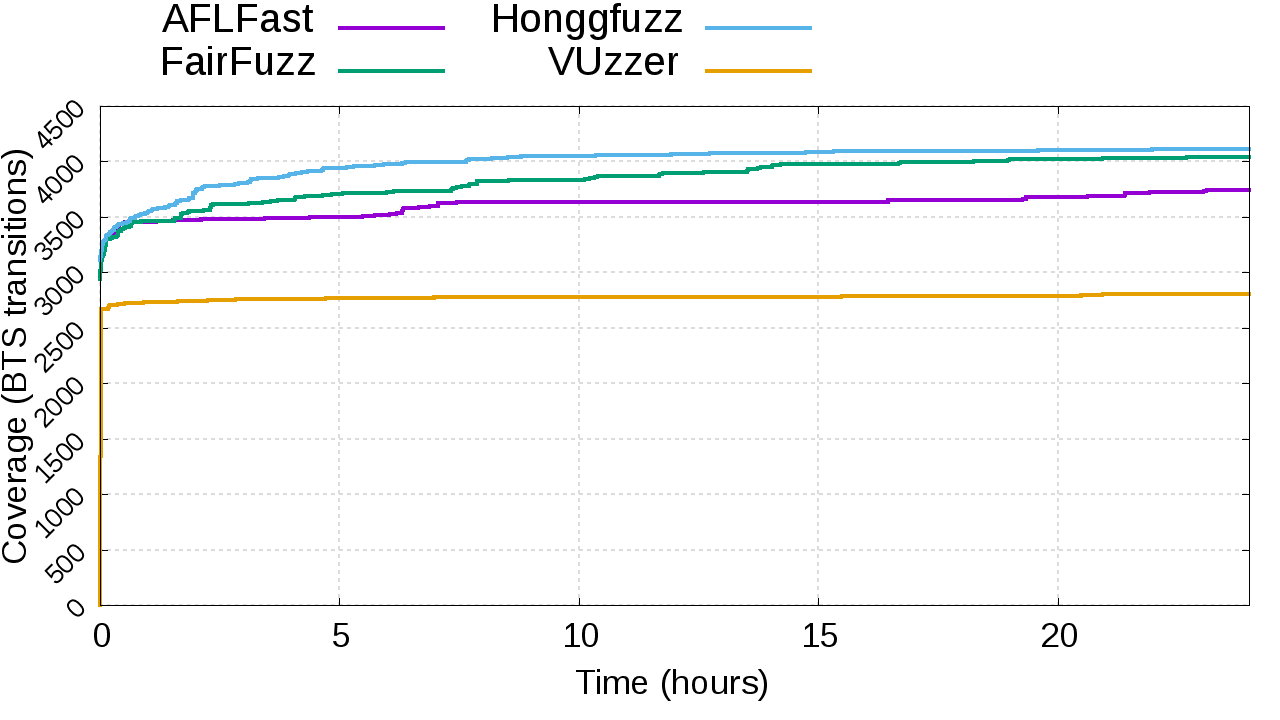
\includegraphics[width=.65\textwidth]{figures/mono-djpeg}
            \label{fig:eval-mono-djpeg}
        }
        \subfloat[\objdump]{%
            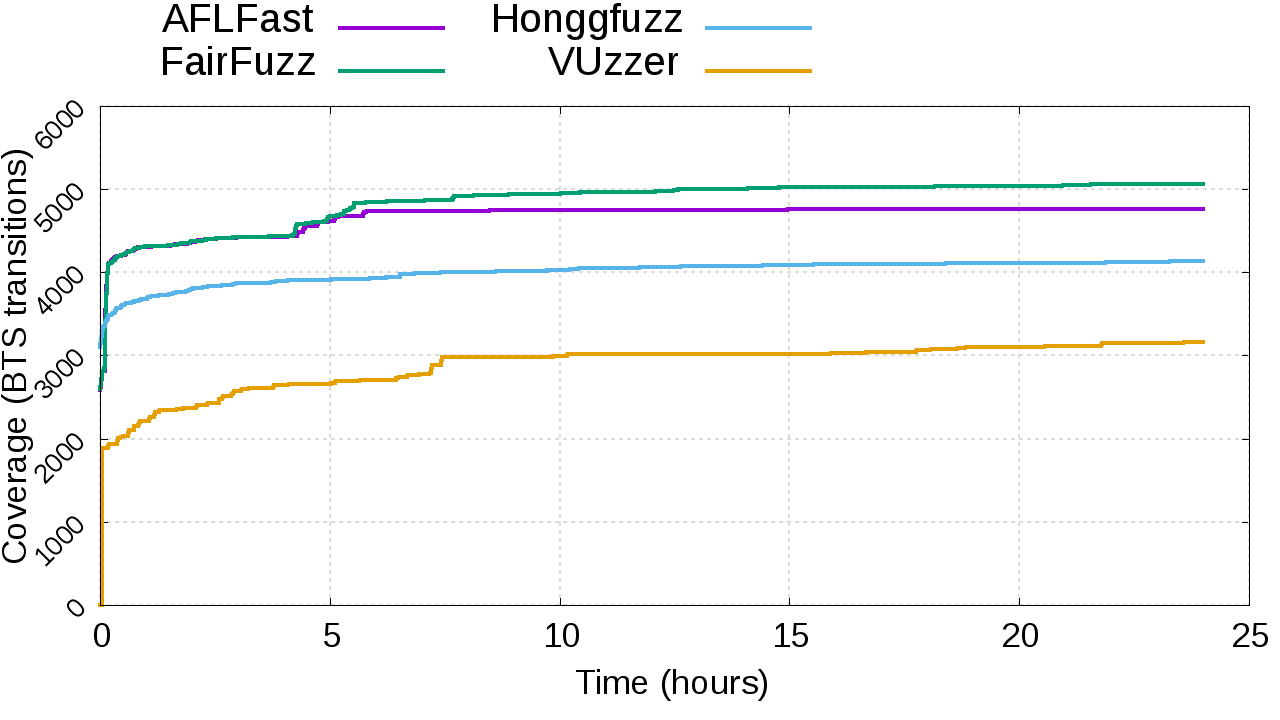
\includegraphics[width=.65\textwidth]{figures/mono-objdump}
            \label{fig:eval-mono-objdump}
        }
    \end{adjustbox}
    \begin{adjustbox}{center}
        \subfloat[\tiffpdf]{%
            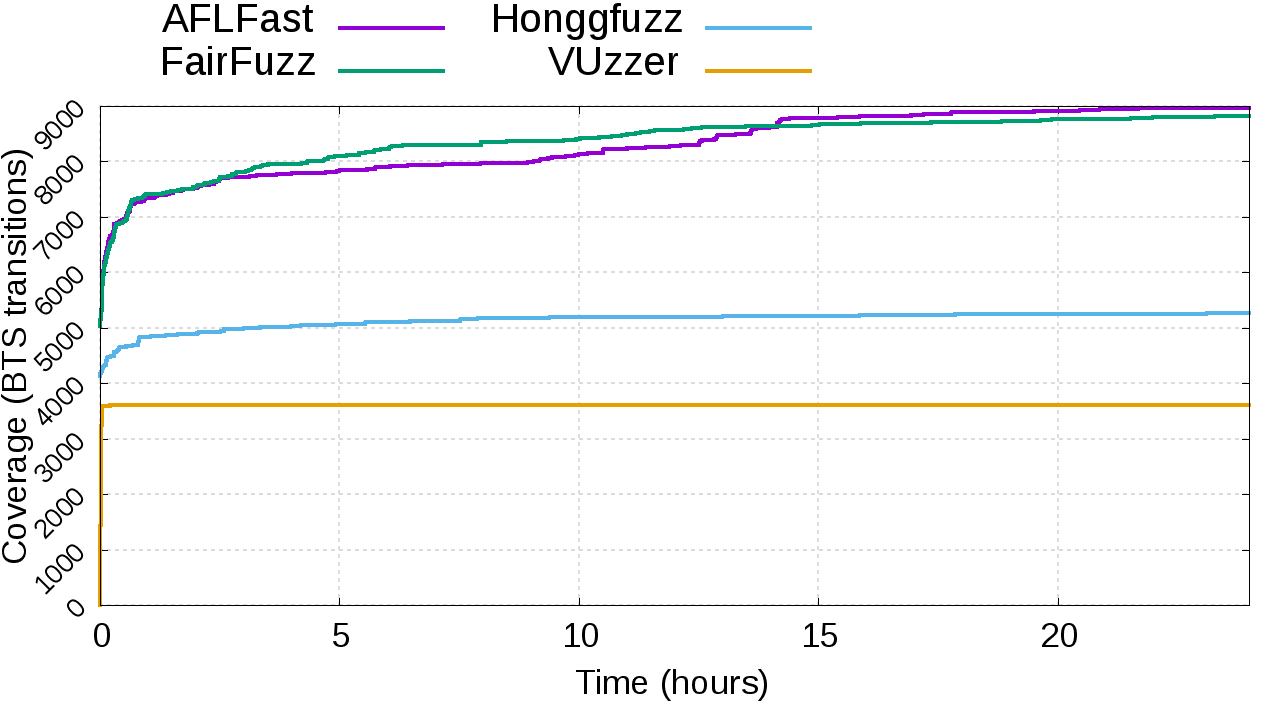
\includegraphics[width=.65\textwidth]{figures/mono-tiff2pdf}
            \label{fig:eval-mono-tiff2pdf}
        }
        \subfloat[\listswf]{%
            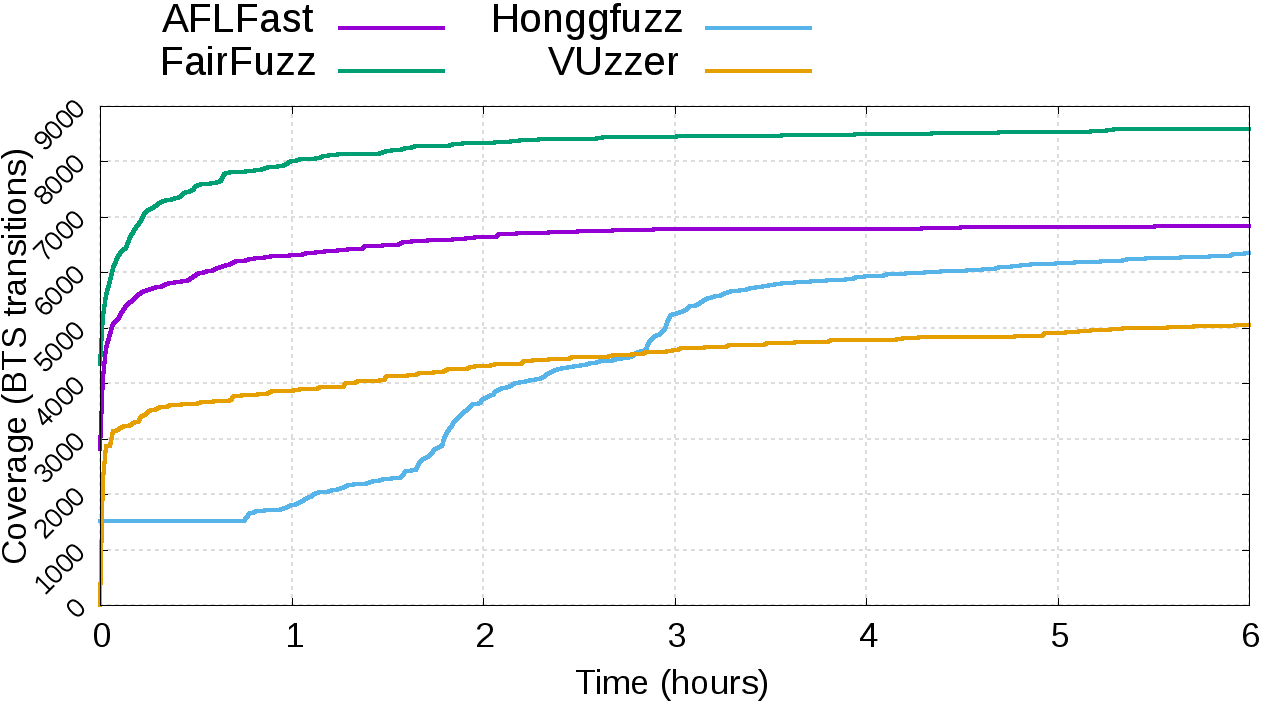
\includegraphics[width=.65\textwidth]{figures/mono-ming}
            \label{fig:eval-mono-ming}
        }
    \end{adjustbox}
    \caption{Mean coverage over time for single fuzzers.}
    \label{fig:eval-mono}
\end{figure}

To derive more robust and meaningful insights over these results, we employ the
Bayesian estimation model proposed in~\cite{kruschke2013bayesian}. This model
provides, among others, estimates of the posterior distributions of the means
and their differences of two given sets of observations.
Figure~\ref{fig:djpeg-means} shows the distribution of the difference of means
of \honggfuzz\ against \aflfast\ and \fairfuzz\ for \djpeg. The figure also
shows the $95\%$ \ac{HDI}, which represents the interval of values onto which
$95\%$ of the probability mass lies. Figure~\ref{fig:djpeg-m-hongg-afl} clearly
shows that the \ac{HDI} lies completely above zero, meaning that with high
credibility we can say that \honggfuzz\ performs better than \aflfast\ over
\djpeg. Unfortunately the same conclusion cannot be made for the comparison of
\honggfuzz\ against \fairfuzz. Figure~\ref{fig:djpeg-m-hongg-fair} shows that a
difference of means of zero lies on the \ac{HDI}; moreover an estimated $20.2\%$
of the probability mass lies below zero (\ie~in favor of \fairfuzz).

\begin{figure}[h]
    \centering%
    \subfloat[\honggfuzz\ vs.\ \aflfast]{%
        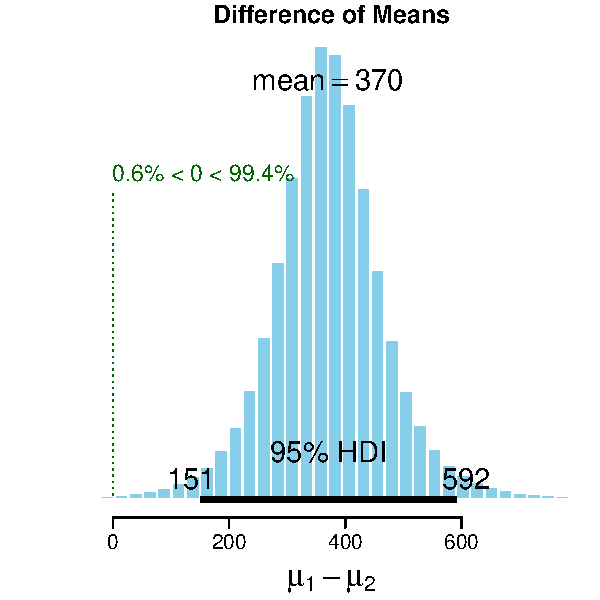
\includegraphics[width=.5\textwidth]{figures/cropped/djpeg-m-hongg-afl}
        \label{fig:djpeg-m-hongg-afl}
    }
    \subfloat[\honggfuzz\ vs.\ \fairfuzz]{%
        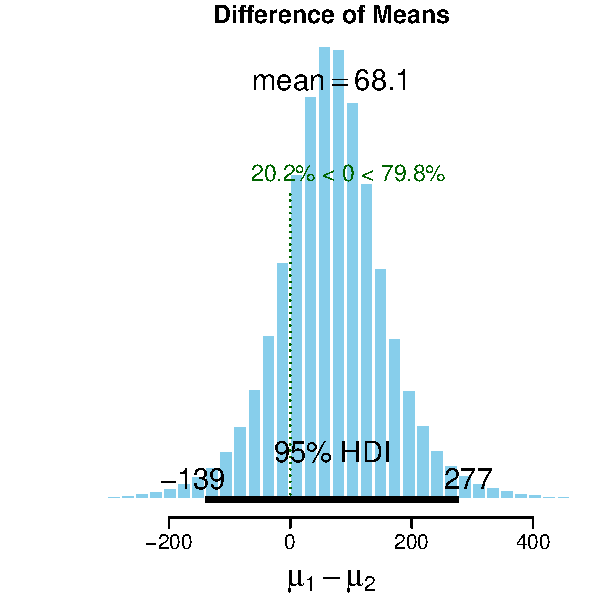
\includegraphics[width=.5\textwidth]{figures/cropped/djpeg-m-hongg-fair}
        \label{fig:djpeg-m-hongg-fair}
    }
    \caption{Single fuzzers: distribution of difference of means for \djpeg.}
    \label{fig:djpeg-means}
\end{figure}

Figure~\ref{fig:objdump-means} shows the difference of means for \objdump. For
both the cases of \fairfuzz\ against \aflfast\
(Figure~\ref{fig:objdump-m-fair-afl}) and \fairfuzz\ against \honggfuzz\
(Figure~\ref{fig:objdump-m-fair-hongg}) the results strongly support the claim
of \fairfuzz\ uncovering more basic block transitions for \objdump.

\begin{figure}[h]
    \centering%
    \subfloat[\fairfuzz\ vs.\ \aflfast]{%
        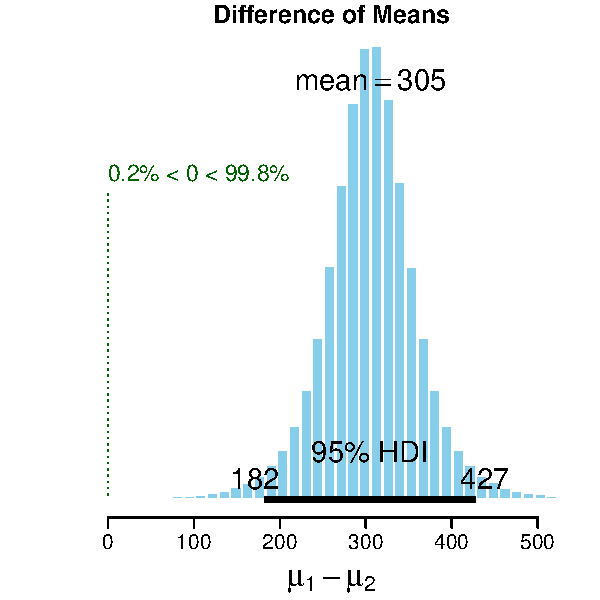
\includegraphics[width=.5\textwidth]{figures/cropped/objdump-m-fair-afl}
        \label{fig:objdump-m-fair-afl}
    }
    \subfloat[\fairfuzz\ vs.\ \honggfuzz]{%
        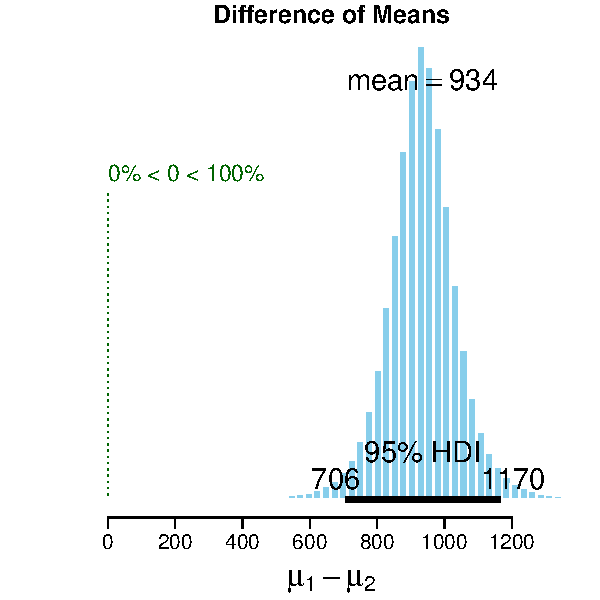
\includegraphics[width=.5\textwidth]{figures/cropped/objdump-m-fair-hongg}
        \label{fig:objdump-m-fair-hongg}
    }
    \caption{Single fuzzers: distribution of difference of means for \objdump.}
    \label{fig:objdump-means}
\end{figure}

Figure~\ref{fig:tiff2pdf-means} shows the difference of means for \tiffpdf.
Unfortunately, as for \djpeg, we are not able to decisively confirm whether
\aflfast\ is better than \fairfuzz\ (Figure~\ref{fig:tiff2pdf-m-afl-fair}). We
can be instead more certain affirming that \aflfast\ outperforms \honggfuzz\ for
the given \sut\ (Figure~\ref{fig:tiff2pdf-m-afl-hongg}).

\begin{figure}[h]
    \centering%
    \subfloat[\aflfast\ vs.\ \fairfuzz]{%
        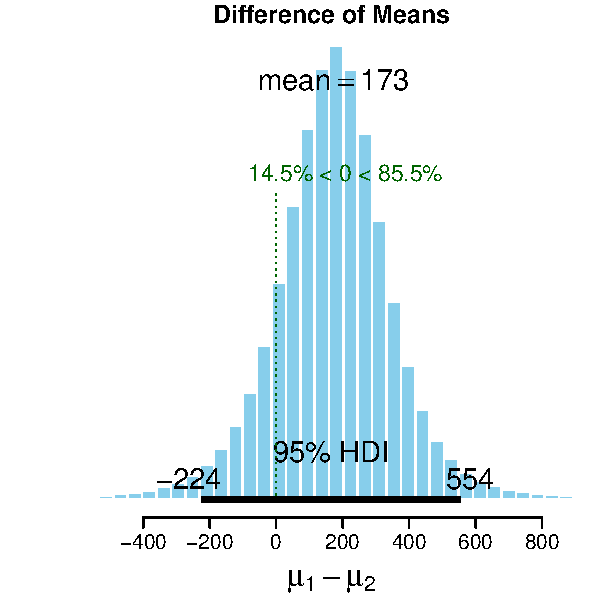
\includegraphics[width=.5\textwidth]{figures/cropped/tiff2pdf-m-afl-fair}
        \label{fig:tiff2pdf-m-afl-fair}
    }
    \subfloat[\aflfast\ vs.\ \honggfuzz]{%
        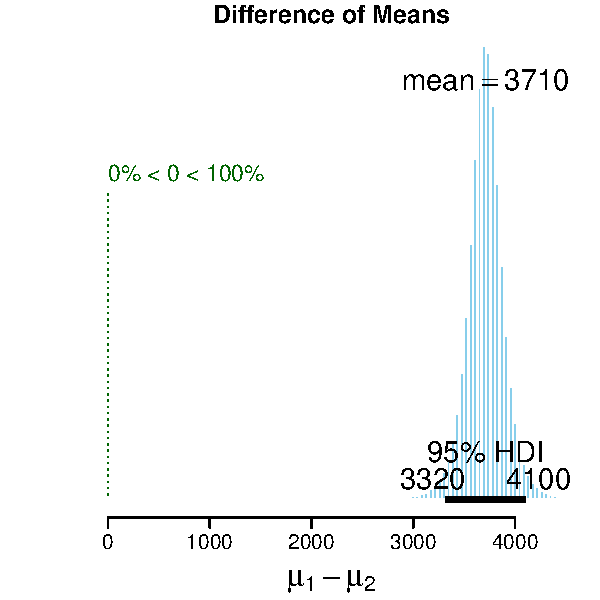
\includegraphics[width=.5\textwidth]{figures/cropped/tiff2pdf-m-afl-hongg}
        \label{fig:tiff2pdf-m-afl-hongg}
    }
    \caption{Single fuzzers: distribution of difference of means for \tiffpdf.}
    \label{fig:tiff2pdf-means}
\end{figure}

To validate differences among fuzzers even further, we compare, in
Table~\ref{tab:eval-mono-union}, the best single fuzzer with the result of
taking the union of coverage traces across all four fuzzers for each time step.
For this comparison we use a time limit of $6$ hours, to align it with the
evaluations presented in the following Section~\ref{sec:eval-coop}. The table
clearly shows that fuzzers uncover unique basic block transitions that are not
exposed by any other fuzzer (\ie~uncover disjoint sets of transitions) and this
contributes to reaching an higher final coverage consistently across all
examined programs.

\begin{table}[h]
    \centering%
    \begin{tabular}{l c l c}
        \textbf{\sut} & \multicolumn{2}{c}{\textbf{best single}} & \textbf{union} \\
        \bottomrule%
        \djpeg& $3975.4 \pm 67.1442$ & \honggfuzz& \hicell$4028.6 \pm 47.7396$ \\
        \objdump& $4840.4 \pm 12.7867$ & \fairfuzz& \hicell$5035.6 \pm 54.5944$ \\
        \tiffpdf& $8224.6 \pm 254.638$ & \fairfuzz& \hicell$8623.2 \pm 183.399$ \\
        \listswf& $8586.8 \pm 87.7467$ & \fairfuzz& \hicell$8916.6 \pm 83.8381$
    \end{tabular}
    \caption{Mean coverage with $95\%$ confidence intervals for best single
    fuzzer and union of coverage traces.}
    \label{tab:eval-mono-union}
\end{table}

\section{Cooperative Fuzzing Evaluation}
\label{sec:eval-coop}

In this section we present an evaluation of the efficacy of cooperation.
Table~\ref{tab:eval-coop} presents the result of running the \ac{CFF} for $6$
hours against the union of coverage traces, reported for convenience from
Table~\ref{tab:eval-mono-union}.

\begin{table}[h]
    \centering%
    \begin{tabular}{l c c c}
        \textbf{\sut} & \textbf{multi} & \textbf{single} & \textbf{union} \\
        \bottomrule%
        \djpeg& $4056.4 \pm 76.9499$ & \hicell$4078.4 \pm 85.6738$ & $4028.6 \pm 47.7396$ \\
        \objdump& $5414.6 \pm 224.121$ & \hicell$5529.6 \pm 338.651$ & $5035.6 \pm 54.5944$ \\
        \tiffpdf& \hicell$8765.6 \pm 183.682$ & $8577.6 \pm 99.2457$ & $8623.2 \pm 183.399$ \\
        \listswf& \hicell$9008.4 \pm 122.81$ & $8801.4 \pm 96.4045$ & $8916.6 \pm 83.8381$
    \end{tabular}
    \caption{Mean coverage with $95\%$ confidence intervals for winning
    strategies that select single or multiple winners and without cooperation.}
    \label{tab:eval-coop}
\end{table}

\begin{figure}[t]
    \centering%
    \begin{adjustbox}{center}
        \subfloat[\djpeg]{%
            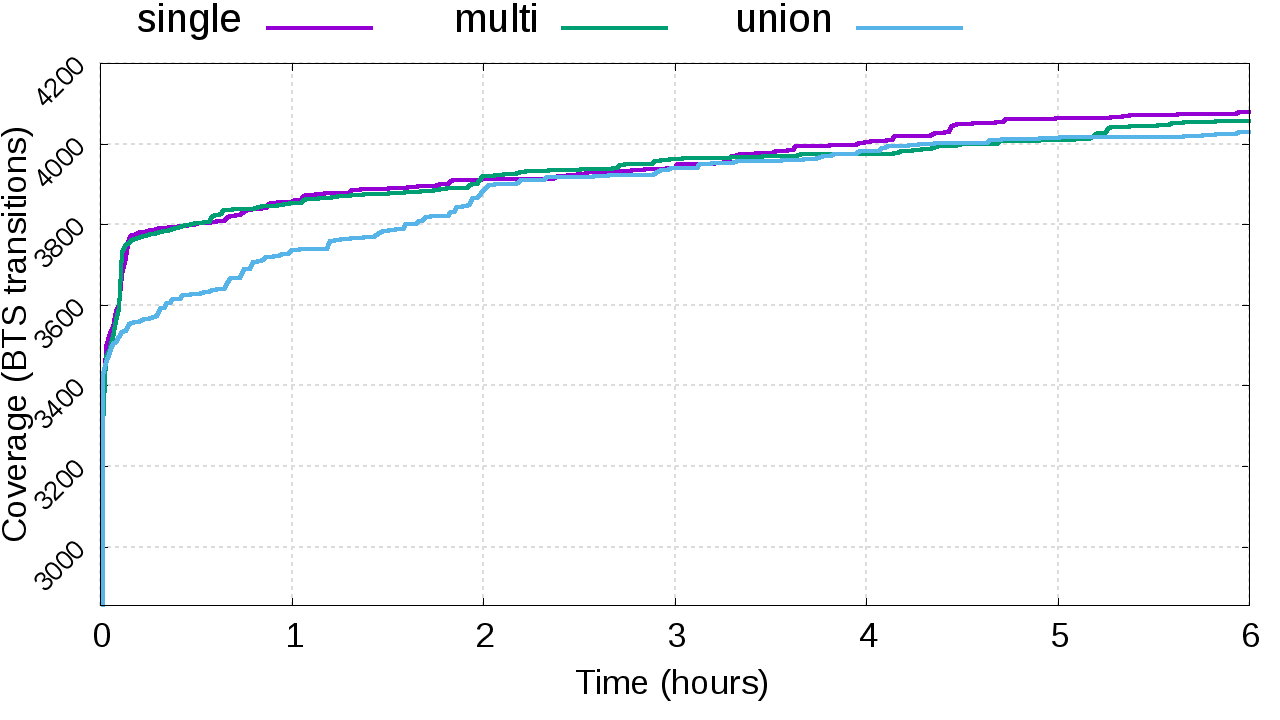
\includegraphics[width=.65\textwidth]{figures/vs-djpeg}
            \label{fig:eval-coop-djpeg}
        }
        \subfloat[\objdump]{%
            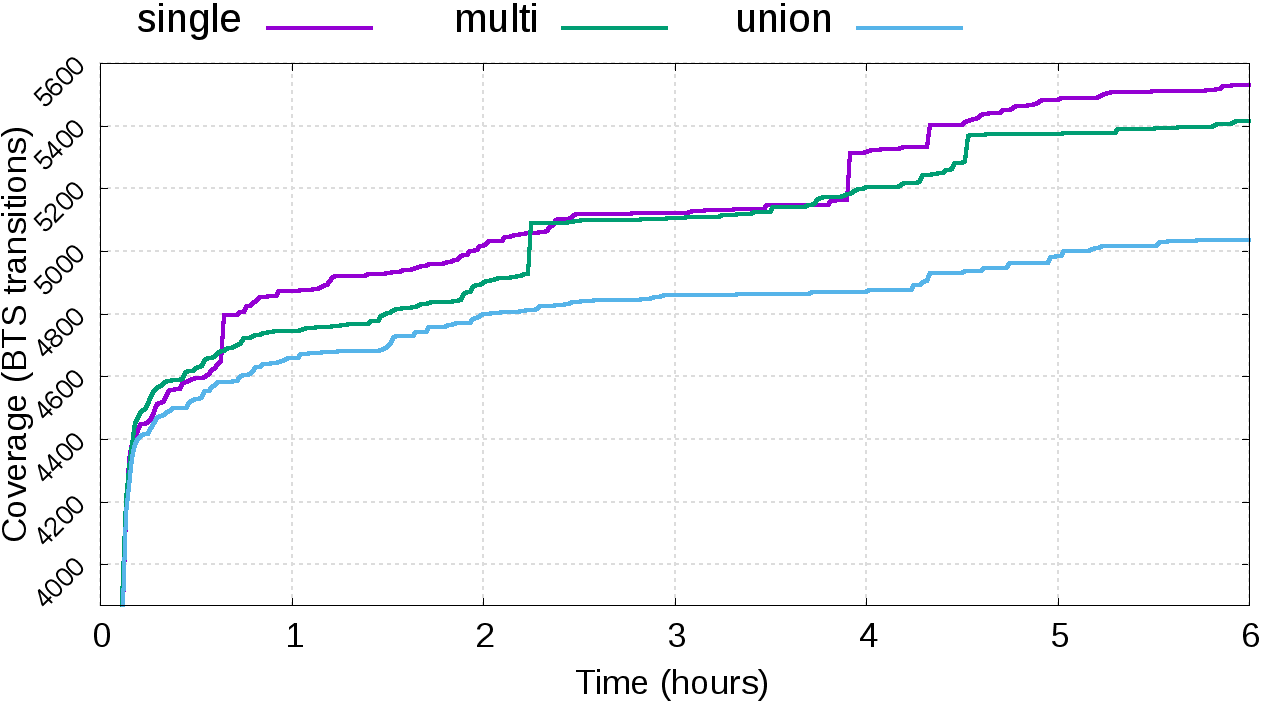
\includegraphics[width=.65\textwidth]{figures/vs-objdump}
            \label{fig:eval-coop-objdump}
        }
    \end{adjustbox}
    \begin{adjustbox}{center}
        \subfloat[\tiffpdf]{%
            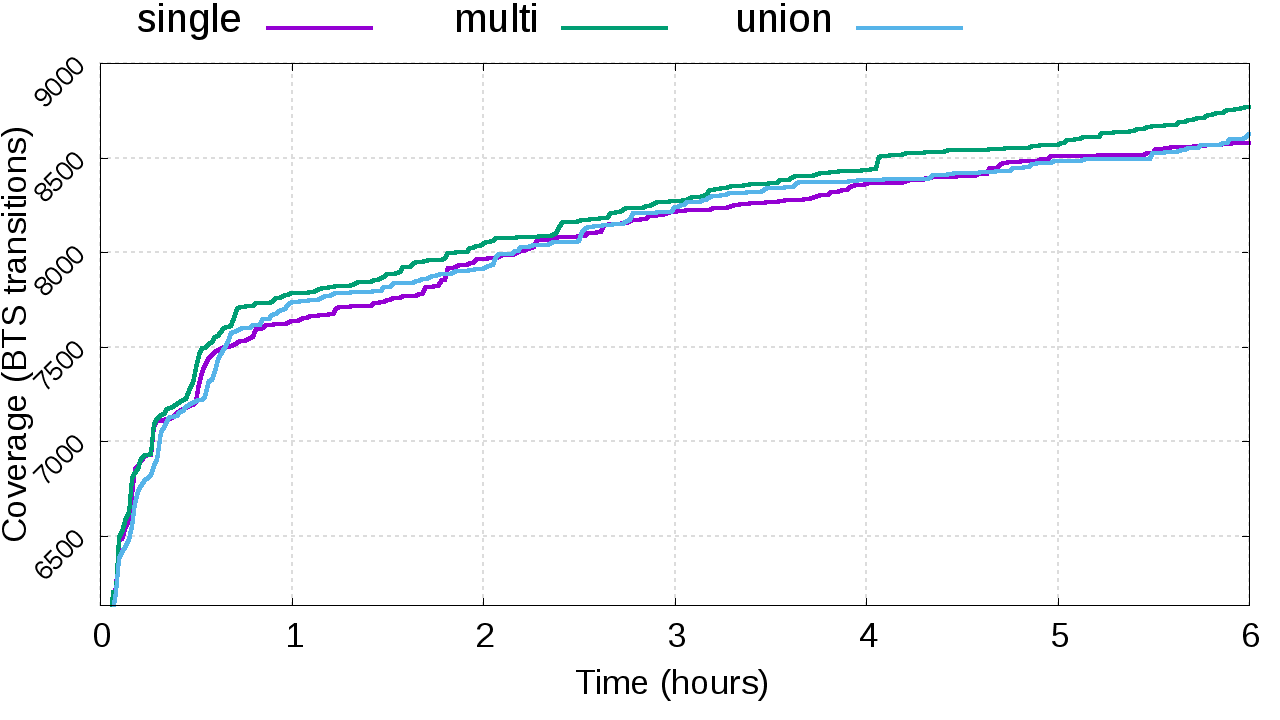
\includegraphics[width=.65\textwidth]{figures/vs-tiff2pdf}
            \label{fig:eval-coop-tiff2pdf}
        }
        \subfloat[\listswf]{%
            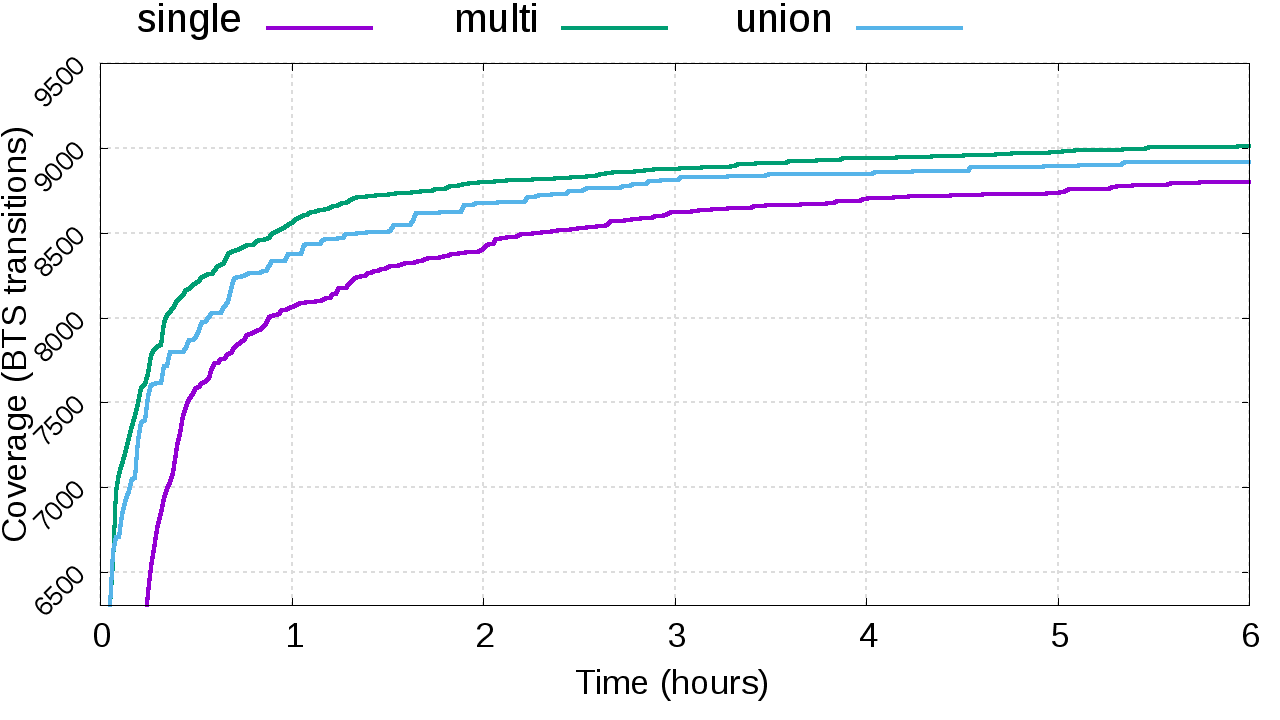
\includegraphics[width=.65\textwidth]{figures/vs-ming}
            \label{fig:eval-coop-ming}
        }
    \end{adjustbox}
    \caption{Eval coop}
    \label{fig:eval-coop}
\end{figure}

\section{Crash Analysis}


%\include{multiToC} % <--- just debug stuff, ignore for your documents
% ********************************************************************
% Backmatter
%*******************************************************
\appendix
%\renewcommand{\thechapter}{\alph{chapter}}
\cleardoublepage
\chapter{Appendix}
\lipsum


%********************************************************************
% Other Stuff in the Back
%*******************************************************
\cleardoublepage%********************************************************************
% Bibliography
%*******************************************************
% work-around to have small caps also here in the headline
% https://tex.stackexchange.com/questions/188126/wrong-header-in-bibliography-classicthesis
% Thanks to Enrico Gregorio
\defbibheading{bibintoc}[\bibname]{%
  \phantomsection
  \manualmark
  \markboth{\spacedlowsmallcaps{#1}}{\spacedlowsmallcaps{#1}}%
  \addtocontents{toc}{\protect\vspace{\beforebibskip}}%
  \addcontentsline{toc}{chapter}{\tocEntry{#1}}%
  \chapter*{#1}%
}
\printbibliography[heading=bibintoc]

% Old version, will be removed later
% work-around to have small caps also here in the headline
%\manualmark
%\markboth{\spacedlowsmallcaps{\bibname}}{\spacedlowsmallcaps{\bibname}} % work-around to have small caps also
%\phantomsection
%\refstepcounter{dummy}
%\addtocontents{toc}{\protect\vspace{\beforebibskip}} % to have the bib a bit from the rest in the toc
%\addcontentsline{toc}{chapter}{\tocEntry{\bibname}}
%\label{app:bibliography}
%\printbibliography

% ********************************************************************
% Game Over: Restore, Restart, or Quit?
%*******************************************************
\end{document}
% ********************************************************************
